
In \ref{intermediate} we brought up the variety $\mathbb{G}$ of \emph{Gödel algebras} as the algebraic semantics of Gödel-Dummett (Propositional) Logic $\mathcal{G}$. \newline
We saw that \emph{finite-valued} Gödel-Dummett Logic $\mathcal{G}_n$ has a semantic characterization given by the n-chains $\emph{C}_n$. \newline
In fact, if we take the \emph{subdirect} product of k-chains with $k \leq n$, the resulting \emph{sub-variety} is called $\mathbb{G}_n$ or \emph{n-valued Gödel algebras} which model the logic $\mathcal{G}_n$. \newline
Using a Stone-like \emph{Duality} between \emph{finite} Gödel algebras and a soon to be introduced category of \emph{Finite Forests} we aim to explore the Topos semantics of a sub-category of \emph{Bushes} and \emph{re-discover} our target logic $\mathcal{G}_3$ at the propositional and first-order levels. 
\newline
We start by giving the following introduction to \emph{Finite Forests} and their duality with \emph{Finite Gödel algebras} building on the works of \cite{towards}, \cite{manyval}, \cite{recursive} and \cite{computing} among others.

\newpage
\section{Finite Forests}
\label{chapter02}

\subsection{First Steps}

We need the following preliminary definitions:

\begin{definition}[\emph{down-set} of $S\subseteq F$] 
	$\downarrow S := \{ x \in F \;|\; x \leq y \text{ for some } y\in S \}$.
\end{definition}

\begin{definition}[\emph{up-set} of $S\subseteq F$] 
	$\uparrow S := \{ x \in F \;|\; x \geq y \text{ for some } y\in S \}$.
\end{definition}

Now, what do we mean by \emph{finite forests}? 

\begin{definition}[\emph{finite forest F}]
	\emph{F} is a finite poset in which the \emph{down-set} of each element $x \in F$, i.e., $ \downarrow x :=  \downarrow \{x\} $ is a \emph{chain}\footnote{totally ordered sub-poset.} with the order inherited from \emph{F}.
\end{definition}

\begin{definition}[\emph{finite tree T}]
	$T$ is a finite forest with a minimum element called \emph{root} or \emph{bottom}.
\end{definition}

\begin{definition}[\emph{sub-forest G}] 
	A sub-forest $G$ of a finite forest $F$ is a \emph{downward-closed sub-poset G of F}, i.e., $G=\downarrow G$.\newline $F$ in this case is also called a \emph{super-forest} of the finite forest $G$.
\end{definition}

\begin{figure}[h]
	\centering
	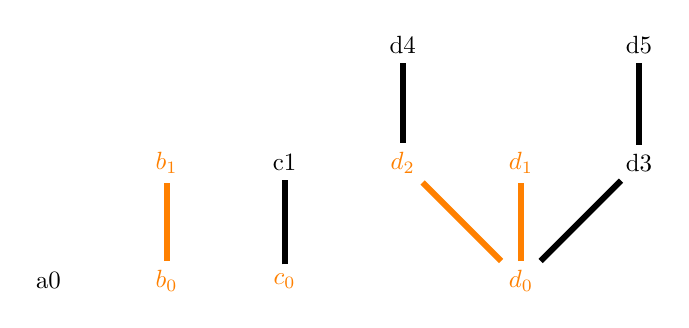
\begin{tikzpicture}[thick,scale=0.5, every node/.style={scale=0.9}]
		\node (A)  at (0,0) {a0};
		\node (B)  at (3,0) {\textcolor{orange}{$b_0$}};
		\node (C)  at (3,3) {\textcolor{orange}{$b_1$}};
		\node (D)  at (6,0) {\textcolor{orange}{$c_0$}};
		\node (E)  at (6,3) {c1};
		\node (F)  at (12,0) {\textcolor{orange}{$d_0$}};
		\node (G)  at (12,3) {\textcolor{orange}{$d_1$}};
		\node (H)  at (9,3) {\textcolor{orange}{$d_2$}};
		\node (I)  at (15,3) {d3};
		\node (J)  at (9,6) {d4};
		\node (K)  at (15,6) {d5};
		\draw[line width=.03in, orange] (B) -- (C);
		\draw[line width=.03in] (D) -- (E);
		\draw[line width=.03in, orange] (F) -- (G);
		\draw[line width=.03in, orange] (F) -- (H);
		\draw[line width=.03in] (F) -- (I);
		\draw[line width=.03in] (H) -- (J);
		\draw[line width=.03in] (I) -- (K);
	\end{tikzpicture}
	\caption{A finite forest \emph{F} and its sub-forest \textcolor{orange}{$G$} in which the nodes are ordered bottom to top and displayed accordingly. \newline The figure is meant to represent the finite poset\newline $F = \{ a_0,\; b_0 < b_1,\; c_0 < c_1,\; d_0 < d_1 < d_4,\; d_0 < d_2,\; d_0 < d_3 < d_5 \}$ and its sub-forest \newline $\textcolor{orange}{G}=\{ \textcolor{orange}{b_0} < \textcolor{orange}{b_1},\; \textcolor{orange}{c_0},\; \textcolor{orange}{d_0} < \textcolor{orange}{d_1},\;\textcolor{orange}{d_0} < \textcolor{orange}{d_2}\}$.  }
\end{figure}

\newpage
\subsection{The Categories $ \mathbb{FF}_*$}

From now on a slight abuse of notation will be used: "$C\in \mathbb{C}$" instead of "object $C$ in $\mathbb{C}$".
\newline
We introduce appropriate \emph{morphisms} or \emph{arrows} between finite forests \emph{F} and \emph{G} in the form of \emph{order-preserving open maps}:
\begin{definition}[\emph{open map}]
	A map $ f: F \rightarrow G $ is \emph{open} if it carries any down-set of $ S \subseteq F $ to a down-set of $ T \subseteq G $ :$f(\downarrow S) = (\downarrow T)$.
\end{definition}

\begin{remark}
	$f(\downarrow S) = (\downarrow T)$ is equivalent to $\forall x \in F : f(\downarrow x) = \downarrow f(x)$. 
\end{remark}

\begin{figure}[h] 
	\centering
	\begin{tikzpicture}[thick,scale=0.5, every node/.style={scale=0.9}]
		\node (A) at (0,0) {\textcolor{red}{$a_0$}};
		\node (B) at (3,0) {\textcolor{OliveGreen}{$b_0$}};
		\node (C) at (3,3) {\textcolor{SkyBlue}{$b_1$}};
		\node (D) at (6,0) {\textcolor{red}{$c_0$}};
		\node (E) at (6,3) {\textcolor{red}{$c_1$}};
		\node (F) at (12,0) {\textcolor{OliveGreen}{$d_0$}};
		\node (G) at (12,3) {\textcolor{SkyBlue}{$d_2$}};
		\node (H) at (9,3) {\textcolor{OliveGreen}{$d_1$}};
		\node (I) at (15,3) {\textcolor{SkyBlue}{$d_3$}};
		\node (J) at (9,6) {\textcolor{SkyBlue}{$d_4$}};
		\node (K) at (15,6) {\textcolor{SkyBlue}{$d_5$}};
		
		\node (u) at (16,1) {};
		\node (v) at (22,1) {};
		
		\node (L) at (23,0) {\textcolor{red}{$e_0$}};
		\node (M) at (26,0) {\textcolor{OliveGreen}{$f_0$}};
		\node (N) at (26,3) {\textcolor{SkyBlue}{$f_1$}};
		
	\draw[->, dotted, line width=.01in] (u) -- node[anchor=north] {$h$} (v);
	
		\draw[line width=.03in, SkyBlue] (B) -- (C);
		\draw[line width=.03in, red] (D) -- (E);
		\draw[line width=.03in, SkyBlue] (F) -- (G);
		\draw[line width=.03in,OliveGreen] (F) -- (H);
		\draw[line width=.03in, SkyBlue] (F) -- (I);
		\draw[line width=.03in, SkyBlue] (H) -- (J);
		\draw[line width=.03in, SkyBlue] (I) -- (K);
		
		\draw[line width=.03in, SkyBlue] (M) -- (N);
	\end{tikzpicture}
	\caption{An arrow $h$ between forests \emph{F} (left) and \emph{G} (right). \newline
		The nodes of \emph{F} are mapped to the nodes of corresponding color in \emph{G}. \newline For example $a_0, b_0 \mapsto f_0$ and $b_1 \mapsto f_1$.}
\label{fig:arrow}
\end{figure}
 

	We define the category in question:
	\begin{definition}[category $\mathbb{FF}$]
		$\mathbb{FF}$ is the category formed by taking finite forests as objects and order-preserving open maps as arrows.
	\end{definition}
	Of particular interest to us are finite forests of \emph{height} at most $n \geq 0$.
	
	\begin{definition}[\emph{height}]
	The \emph{height} of a finite forest \emph{F} is the maximum cardinality of a downset $\downarrow x$ for $ x \in F$.
	\end{definition} 
	
	In the example \emph{F} in figure~\ref{fig:arrow} has height 3 whilst \emph{G} has height 2. 
	
	\begin{definition}[category $\mathbb{FF}_n$]
		The (full) subcategory $\mathbb{FF}_n$ of $\mathbb{FF}$ has finite forests of height at most $n$ as objects and open maps between them as arrows.\newline
		The objects of $\mathbb{FF}_2$ are called \emph{bushes}.
	\end{definition}
	
	Also the \emph{finite trees} form the subcategory $\mathbb{T}$. \newline\newline
	Let $\mathbb{FF}_*$ stand for either $\mathbb{FF}$ or $\mathbb{FF}_n$ for $n>0$.
	\newline
	The following properties are valid  in $\mathbb{FF}_*$: \footnote{here we omit to verify that these constructions satisfy the categorical properties of Terminal and Initial objects, Products, Co-products and so on. For reference see \cite{towards} \& \cite{recursive}.}
	
	\begin{thm}[Terminal]
		The \emph{terminal} object is given by the singleton forest denoted as $\textbf{1} := \{ \bullet \}$.
	\end{thm}
	 
	 \begin{thm}[Initial]
	 	The \emph{initial} object is given by the empty forest denoted as $\textbf{0} := \{\}$.
	 \end{thm} 

The \emph{Co-product} or \emph{Sum} between two forests $F$ and $G$ is readily given. 

\begin{figure}[h]
	\centering
	\begin{tikzpicture}[thick,scale=0.8, every node/.style={scale=0.9}]
		\node (A)  at (0,0) {$\bigcdot$};
		\node (B)  at (3,0) {$\bot$};
		\node (C)  at (3,3) {$\bigcdot$};
		
		\draw[line width=.01in] (B) -- (C);
		
	\end{tikzpicture}
	\caption{$\Omega$.}
	\label{fig:Omega}
\end{figure}


\begin{thm}[Co-product]
	The \emph{Co-product} $F+G$ between $F$ and $G$ is obtained by taking the \emph{disjoint union} of the two posets and the inclusion maps $\iota_F : F \hookrightarrow F+G$ and $\iota_G : G \hookrightarrow F+G $. 
\end{thm}

For example $\Omega := \textbf{1} + \textbf{1}_{\bot}$ is displayed in figure~\ref{fig:Omega}.


\begin{cor}
	Each forest $F$ in $\mathbb{FF}_*$ uniquely determines a finite family of trees $\{F_i\}_{i=1}^N$ such that $F = \sum_{i=1}^{N} F_i$. \footnote{by $\sum$ we mean the coproduct of the summands.}
\end{cor}

	
\newpage

Now for each finite forest $F$ we write $F_{\bot}$ as the tree obtained by appending a new bottom/root element as the new minimum.\newline 
In fact:
\begin{remark}
	every tree $T$ is of the form $T = T'_{\bot}$ for some finite forest $T'$.
\end{remark}

(Abuse of notation: oftentimes "$=$" in these cases is used instead of "$\cong$"). \newline
In $\mathbb{FF}$ the \emph{product} $F \times G$ between $F$ and $G$ is defined in a recursive manner \newline
We require the following properties to hold for our product:
\begin{lem} ${}$
	\begin{itemize}
		\item ($\times$ by \textbf{0} is \textbf{0}) $\forall F$: $F \times \textbf{0} = \textbf{0} = \textbf{0} \times F$  
		\item (\textbf{1} as neutral element of $\times$) $\forall F$: $F \times \textbf{1} = F = \textbf{1} \times F$
		\item (distributive law for $\times$) $\forall F,G,H $: $ F \times (G+H) = (F \times G) + (F \times H) $
	\end{itemize}
\end{lem}
The recursive formula for $F_{\bot} \times G_{\bot} $ is given by:
\begin{definition}[Product]
	\begin{equation}
		F_{\bot} \times G_{\bot} := ( (F \times G_{\bot}) + ( F \times G ) + (F_{\bot} \times G) )_{\bot}
	\end{equation}
\end{definition}
 The projection maps are also given recursively following the construction of the product object :
 	\begin{definition}[Projections]
 		The maps $ \pi_{F_\bot} : 	F_{\bot} \times G_{\bot} \twoheadrightarrow F_{\bot}$ and $\pi_{G_\bot} : F_{\bot} \times G_{\bot} \twoheadrightarrow G_{\bot} $ are defined as follows:
 		\newline
 		Let $t_0$ be the root of $F_{\bot} \times G_{\bot}$ and $r_0,s_0$ the roots respectively of $F_{\bot}$ and $G_{\bot}$.
 		\begin{gather*}
 			\pi_{F_\bot}: t_0 \mapsto r_0 \\
 			\pi_{G_\bot} : t_0 \mapsto s_0 
 		\end{gather*}
 		Let $F_0$ and $G_0$ stand for $F_\bot$ and $G_\bot$. \newline 
 		Recalling the representation of each finite forest as a finite sum of trees, $F_\bot = (\sum_{i=1}^{N} F_i)_\bot$ and $G_\bot = (\sum_{j=1}^{M} G_j)_\bot$.\newline
 		Each element $x \in  (F \times G_0) + ( F \times G ) + (F_0 \times G) $ belongs to a unique tree $F_i \times G_j$ with $(i+j) >0$.\newline
 		Also let $\iota_{F_i} : F_i \hookrightarrow F_\bot$ the set-inclusion of the support of $F_i$ into $F_\bot$  and $\iota_{G_j}$ the analogous map for $G_j$. Then:
 		\begin{gather*}
 			\pi_{F_\bot}: x \mapsto \iota_{F_i} ( \pi_{F_i}(x) ) \\
 			\pi_{G_\bot}: x \mapsto \iota_{G_j} ( \pi_{G_j}(x) ) 
 		\end{gather*}
 	\end{definition}
 	
 	\begin{lem}
 			The object $F_{\bot} \times G_{\bot}$ together with $\pi_{F_\bot}$ and $\pi_{G_\bot}$ is proven in \cite{recursive} to be the desired product object in $\mathbb{FF}$ together with the associated projections.
 	\end{lem}
 
 \begin{figure}[h]
 	\centering
 	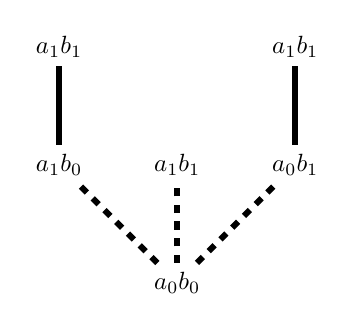
\begin{tikzpicture}[thick,scale=0.5, every node/.style={scale=0.9}]
 		\node (A)  at (0,0) {$a_1b_0$};
 		\node (B)  at (0,3) {$a_1b_1$};
 		\node (C)  at (3,0) {$a_1b_1$};
 		\node (D)  at (6,0) {$a_0b_1$};
 		\node (E)  at (6,3) {$a_1b_1$};
 		\node (F)  at (3,-3) {$a_0b_0$};
 		
 		\draw[line width=.03in] (A) -- (B);
 		\draw[line width=.03in] (D) -- (E);
 		\draw [dashed] [ line width=.03in] (F) -- (A);
 		\draw [dashed] [ line width=.03in] (F) -- (C);
 		\draw [dashed] [ line width=.03in] (F) -- (D);
 		
 	\end{tikzpicture}
 	\caption{The product of $1_\bot = \{a_0 < a_1\} = A$ with $1_\bot = \{b_0 < b_1\} = B$ computed following the recursive formula:\newline
 		$ 1_\bot \times 1_\bot = ( (1 \times 1_\bot) + (1 \times 1) + ( 1_\bot \times 1 )  )_\bot = ( 1_\bot + 1 + 1_\bot )_\bot $.\newline The labeling of the nodes specifies the projections: $a_i b_j$ indicates that this node is taken to $a_i$ by the 'left' projection $\pi_{A}$ and to $b_j$ by the 'right' projection $\pi_B$.}
 \end{figure}
 
 Recalling the previous remarks, we have $ F = \sum_{i=1}^{N} F_i $ and $ G = \sum_{j=1}^{M} G_j $ with each $ F_i,  G_j $ being a tree equal to $(F_i')_\bot,  (G_j')_\bot$ for some finite forests $F_i',  G_j'$.
 
 \begin{thm}[Product in $\mathbb{FF}$] 
 	$\forall F,G \in \mathbb{FF}$ such that $ F = \sum_{i=1}^{N} F_i $ and $ G = \sum_{j=1}^{M} G_j $ the product is given recursively as:   \[ F \times_\mathbb{FF} G = \sum_{i,j=1}^{N,M} (F_i')_\bot \times_\mathbb{FF} (G_j')_\bot \] together with the projection maps $\pi_F$ and $\pi_G$ defined as before for each summand.
 \end{thm}
 
 
 The product in $\mathbb{FF}_n$ is obtained by \emph{trimming} the product in $\mathbb{FF}$.
 
 \begin{thm}[Product in $\mathbb{FF}_n$]\label{thm:prodffn}
 	$\forall F, G \in  \mathbb{FF}_n$, \newline $ F \times_{\mathbb{FF}_n} G $ is the sub-forest of all nodes of height $ \leq n $ of $ F \times_\mathbb{FF} G $ together with the projection maps $\pi_F$ and $\pi_G$ \emph{restricted} to $F \times_{\mathbb{FF}_n} G $.
 \end{thm}
 
 (From now on $\times$ will be used usually instead of $\times_\mathbb{FF}$). \newline
 For the purpose of this work we only display selected instances of  products and projections in the following figures.



\begin{figure}[h]
	\centering
	\begin{tikzpicture}[thick,scale=0.5, every node/.style={scale=0.9}]
		
		\node (a) at (0,-2) { };
		\node (b) at (-4,-2) { };
		\draw[->>, dotted, line width=.01in] (a) -- node[anchor=north] {$\pi_{A}$} (b);
		
\node (c) at (6,-2) { };
\node (d) at (10,-2) { };
\draw[->>, dotted, line width=.01in] (c) -- node[anchor=north] {$\pi_{B}$} (d);

\node (a') at (-1,-7) { };
\node (b') at (-4,-5) { };
\draw[->>, dotted, line width=.01in] (a') -- node[anchor=north] {$\pi_{A}'$} (b');

\node (c') at (7,-7) { };
\node (d') at (10,-5) { };
\draw[->>, dotted, line width=.01in] (c') -- node[anchor=north] {$\pi_{B}'$} (d');

	
		\node (A0) at (-6,-5) {\textcolor{purple}{$a_0$}};
		\node (A1) at (-6,-2) {\textcolor{pink}{$a_1$}};
		
		\node (A) at (0,0) {\textcolor{pink}{$\bullet$} \textcolor{blue}{$ \bullet $} };
		\node (B) at (0,3) {\textcolor{pink}{$\bullet$} \textcolor{SkyBlue}{$ \bullet $} };
		\node (C) at (3,0) {\textcolor{pink}{$\bullet$} \textcolor{SkyBlue}{$ \bullet $} };
		\node (D) at (6,0) {\textcolor{purple}{$\bullet$} \textcolor{SkyBlue}{$ \bullet $} };
		\node (E) at (6,3) {\textcolor{pink}{$\bullet$} \textcolor{SkyBlue}{$ \bullet $} };
		\node (F) at (3,-3) {\textcolor{purple}{$\bullet$} \textcolor{blue}{$ \bullet $} };
		
		\node (B0) at (12,-5)  {\textcolor{blue}{$b_0$}};
		\node (B1) at (12,-2) {\textcolor{SkyBlue}{$b_1$}};
		
		\draw[line width=2in, thick] (A0) -- (A1);
		
		\draw[line width=2in, thick] (0,0) -- (0,3);
		\draw[line width=2in, thick] (6,0) -- (6,3);
		\draw [line width=2in, thick] (3,-3) -- (0,0);
		\draw [ line width=2in, thick] (3,-3) -- (3,0);
		\draw [ line width=2in, thick] (3,-3) -- (6,0);
		
		\draw[line width=2in, thick] (B0) -- (B1);
		
		\node (A) at (0,-6) {\textcolor{pink}{$\bullet$} \textcolor{blue}{$ \bullet $} };
		\node (C) at (3,-6) {\textcolor{pink}{$\bullet$} \textcolor{SkyBlue}{$ \bullet $} };
		\node (D) at (6,-6) {\textcolor{purple}{$\bullet$} \textcolor{SkyBlue}{$ \bullet $} };
		\node (F) at (3,-9) {\textcolor{purple}{$\bullet$} \textcolor{blue}{$ \bullet $} };
		
		\draw [line width=2in, thick] (3,-9) -- (0,-6);
		\draw [ line width=2in, thick] (3,-9) -- (3,-6);
		\draw [ line width=2in, thick] (3,-9) -- (6,-6);
	\end{tikzpicture}
	\caption{At each node of the product forest (top center) $ 1_\bot \times_{\mathbb{FF}} 1_\bot$ the color of the left and right dot specifies respectively the projection $\pi_A$ from $ 1_\bot \times_{\mathbb{FF}} 1_\bot$ to  $1_\bot = \{a_0,a_1\}$ (left) and the projection $\pi_B$ from $ 1_\bot \times 1_\bot$ to $1_\bot = \{b_0,b_1\}$ (right).\newline
		Below we have 
		the product forest for $\mathbb{FF}_2 $ (bottom center) $ 1_\bot \times_{\mathbb{FF}_2} 1_\bot$ and the associated projections $\pi_{A}'$ and $\pi_{B}'$.}
		\label{fig:product}
\end{figure}


The product $ F \times G $ of two finite forests $F$ and $G$ is \emph{not} the usual cartesian product of the underlying posets. \newline
In fact the cardinality of the underlying set of the product $ | F \times G | = 6$ in the case of $F$ and $G$ of the form $1_\bot$ is not the product of the cardinalities of $ | F | = 2 $ and $ | G | = 2 $.  \newline
(If the context is specified $\times$ will replace $\times_{\mathbb{FF}_n}$). \newline
In the category of \emph{bushes} $\mathbb{FF}_2$ however the underlying set $ | A \times B | $ of the product of two bushes $A$ and $B$ \emph{is} the cartesian product $| A | \times | B | $ of the underlying sets of $A$ and $B$.\newline In figure figure~\ref{fig:product} we have $4 = | 1_\bot \times 1_\bot | = | 1_\bot | \times | 1_\bot | = 2 \times 2 $.

\newpage
\section{The Duality between Algebras and Forests}

We now consider the category $\mathbb{G}$ of Gödel algebras and their homomorphisms and the full subcategory $\mathbb{G}_{fin}$ of \emph{finite}\footnote{finite cardinality.} Gödel algebras. In turn, for each $ n>0 $ the full subcategory $(\mathbb{G_n})_{fin}$ of $\mathbb{G_n}$ contains the \emph{finite n-valued} algebras. \newline
The remarkable result, essentially due to \emph{A.Horn}\footnote{see also chapter IX \cite{fuzzy}.}, that we shall use henceforth is the \emph{dual equivalence} between the category $\mathbb{FF}$ of Finite Forests and the category $\mathbb{G}_{fin}$ of finite Gödel algebras realized by the contra-variant functors \emph{Spec} and \emph{Sub}.

\begin{thm}[Finite spectral duality for Gödel algebras]
	\[ \mathbb{G}_{fin} \simeq \mathbb{FF}^{\textit{op}} \]
\end{thm}

To see how these functors operate we need to introduce the following notions:
\begin{definition}[proper filter]
	A proper filter $\textfrak{f}$ for a Gödel algebra $\mathbf{A}$: $\emptyset \neq \textfrak{f} \subsetneq \mathbf{A}$ is an up-set of $\mathbf{A}$ closed under \emph{meets} i.e.,  $\forall x,y \in \textfrak{f}: x \land y \in \textfrak{f}$.
\end{definition}
\begin{definition}[prime filter]
	A prime filter $\textfrak{p}$ is a proper filter with $0 \notin \textfrak{p}$ and whenever $ (y \lor z) \in \textfrak{p} $ either $y \in \textfrak{p}$ or $z \in \textfrak{p}$. 
\end{definition}
\begin{definition}[principal filter]
	\textfrak{f} is \emph{principal} if \textfrak{f} = $\uparrow x_\textfrak{f}$ \footnote{$\uparrow x := \{y \in \mathbf{A} \;|\; y \geq x\}$.} for some $x_\textfrak{f} \in \textbf{A}$.
\end{definition}
\begin{definition}[prime spectrum]
	 The set of prime filters of $\mathbf{A}$ is also called the \emph{prime spectrum} of $\mathbf{A}$, a.k.a. $Spec(A)$ and is partially ordered by reverse-inclusion $\supseteq$.
\end{definition}
\begin{definition}[join-irreducible]
	$x \in \mathbf{A} $ is join-irreducible if $x \neq 0$ and whenever $ x= y \lor z $ then either $x=z$ or $x=y$.
\end{definition}

The functor \emph{Spec} assigns to an algebra \textbf{A} the prime spectrum of \textbf{A} with its reverse ordering.\newline The functor \emph{Sub} takes the set of sub-forests of \textbf{F} and forms a finite Gödel algebra with intersection, a new "implication" operator and the empty forest.\newline Both the functors act on morphisms by taking pre-images.

\begin{definition}[Spec]
	$\emph{Spec} : \mathbb{G}_{fin} \rightarrow \mathbb{FF}$ \newline
	\newline
			$	\textbf{A} \longmapsto (\emph{Spec}(\textbf{A})  = \{ \textfrak{p}\subseteq \textbf{A} \;|\; \textfrak{p} \text{ prime filter} \}, \supseteq )$ \newline
				$ \textbf{A} \xrightarrow{f} \textbf{B} \longmapsto Spec(\textbf{B}) \xrightarrow{f^{-1}\{\}} Spec(\textbf{A}) $
\end{definition}

\begin{definition}[Sub]
	$ \emph{Sub} :  \mathbb{FF} \rightarrow \mathbb{G}_{fin}$\newline \newline
	 $\textbf{F} \longmapsto \emph{Sub}(\textbf{F}) = (\{\downarrow G \subseteq F\},\cup,\cap,\Rightarrow,\emptyset ) $ with $ H \Rightarrow G := F \setminus \uparrow(H \setminus G) $. \newline
	 $ \textbf{H} \xrightarrow{h} \textbf{G} \longmapsto Sub(G) \xrightarrow{h^{-1}\{\}} Sub(H) $
\end{definition}

Also, if we restrict the functors to the category of finite n-valued algebras and forests of height n-1:

\begin{thm}
	\[ (\mathbb{G_n})_{fin} \simeq \mathbb{FF}^{\textit{op}}_{n-1} \] 
	For instance: $ (\mathbb{G_3})_{fin} \simeq \mathbb{FF}^{\textit{op}}_{2} $, i.e., the category of bushes.
\end{thm}

We use the following result observed in \cite{recursive}:
\begin{lem}
	In each finite Gödel algebra \textbf{A}, all filters \textfrak{f} are principal. \newline Every prime filter $\mathfrak{p}$ is equal to $\uparrow x_\mathfrak{p}$ for some join-irreducible element $x_\mathfrak{p}$.
\end{lem}

To understand how this duality works we start by taking the dual of the \emph{free} Gödel algebra $\mathcal{F}_1$ on one generator $x$.

\begin{figure}[h]
	\centering
	\begin{tikzpicture}[thick,scale=1.2, every node/.style={scale=0.8}]
		\node (A) at (0,0) {0};
		\node (B) at (1,1) {$\neg x$};
		\node (C) at (-1,1) {$x$};
		\node (D) at (0,2) {$x \lor \neg x$};
		\node (E) at (-2,2) {$\neg\neg x$};
		\node (F) at (-1,3) {1};
		
		\draw[line width=.01in] (A) -- (B);
		\draw[line width=.01in] (A) -- (C);
		\draw[line width=.01in] (B) -- (D);
		\draw[line width=.01in] (C) -- (D);
		\draw[line width=.01in] (C) -- (E);
		\draw[line width=.01in] (D) -- (F);
		\draw[line width=.01in] (E) -- (F);
		
		\node (f) at (3.5,0) {$\uparrow \neg x$};
		\node (t) at (5,0) {$\uparrow x$};
		\node (n) at (5,2) {$\uparrow \neg\neg x$};
		
		\draw[line width=.01in] (t) -- (n);
		
		\node (A') at (10,0) {$\emptyset$};
		\node (B') at (11,1) {$\{ \uparrow\neg x \}$};
		\node (C') at (9,1) {$\{ \uparrow x \}$};
		\node (D') at (10,2) {$\{ \uparrow x, \uparrow\neg x \}$};
		\node (E') at (8,2) {$\{ \uparrow\neg\neg x \}$};
		\node (F') at (9,3) {$ Spec(\mathcal{F}_1) $};

		\draw[line width=.01in] (A') -- (B');
		\draw[line width=.01in] (A') -- (C');
		\draw[line width=.01in] (B') -- (D');
		\draw[line width=.01in] (C') -- (D');
		\draw[line width=.01in] (C') -- (E');
		\draw[line width=.01in] (D') -- (F');
		\draw[line width=.01in] (E') -- (F');
	\end{tikzpicture}
	\caption{ $\mathcal{F}_1$ (left),  Spec($\mathcal{F}_1$)  (center) and Sub(Spec($\mathcal{F}_1$)) (right) }
\end{figure}


Note that $\Omega := \textbf{1} + \textbf{1}_\bot = Spec(\mathcal{F}_1)$. This finite forest will be ubiquitous in the upcoming chapters.
\newline
What this duality tells us is that:
\begin{remark}
	Each finite Gödel algebra \textbf{A} is isomorphic to the Gödel algebra of all sub-forests of  $(Spec(\textbf{A}),\supseteq)$ taken as a finite forest.
\end{remark}

The knowledge of a dual category to the category of Gödel algebras in which products and co-products are readily computed provides us with a valuable tool for the study of the structure of these algebras. For example:
\begin{remark}
	The free algebra on $k>0$ generators  $\mathcal{F}_k = k \cdot [\mathcal{F}_1]$ is the \emph{k-th co-power} \footnote{i.e., the co-product iterated k times over the same object.} of the free algebra on one generator, as such its dual is $ [Spec(\mathcal{F}_1)]^k $ the \emph{k-th power} \footnote{i.e., the product iterated k times over the same object.} of $Spec(\mathcal{F}_1)$.
\end{remark}
 
 	In particular we have: 
 
\begin{remark}
	As a consequence of $ (\mathbb{G_3})_{fin} \simeq \mathbb{FF}^{\textit{op}}_{2}$:
 \[\mathcal{F}_1 \cong Sub(Spec(\mathcal{F}_1)) = Sub(\textbf{1}+\textbf{1}_\bot) = Sub(\Omega).\] 
\end{remark}

%check
In fact, this duality can be seen as a \emph{generalization} of the finite case of \emph{Stone's Representation Theorem} (\cite{stone}) for Boolean algebras whereby \emph{finite Boolean algebras are dually equivalent to finite sets}.
\newline
The latter says that classical propositional logic \emph{CPL} can be seen as the logic of \emph{finite sets}:

\begin{remark}
	A formula $\phi$ of \emph{CPL} seen as a \emph{characteristic function} from a finite set/domain/universe $X$ determines a \emph{subset} $\{x \in X \;|\; \phi(x) = 1\}$ of elements for which \emph{$\phi$ is true}.\newline
	Similarly, a formula $\phi$ of $\mathcal{G}$ determines a \emph{sub-forest} of a finite forest for which \emph{$\phi$ is true}.    
\end{remark}
To be more precise:
\begin{remark}
	For every formula $\phi$ which contains propositional variables $p_1,..,p_n$: \newline
	Finite Forests provide (sound and complete) semantics of Gödel-Dummett Propositional Logic $\mathcal{G}$,  i.e., \footnote{here $\models_{H.A.}$ refers to Heyting algebra validity.}
	\begin{equation*}
		\mathcal{G} \vdash \phi \;\text{ iff }\; Sub(Spec(\mathcal{F}_n)) \models_{H.A.} \phi \;\text{ iff }\; \llbracket \phi \rrbracket_{Sub(Spec(\mathcal{F}_n))}=Spec(\mathcal{F}_n).
	\end{equation*}
\end{remark}


\newpage
Using the same \emph{Stone-style} duality as before we obtain:

\begin{figure}[h]
	\centering
	\begin{tikzpicture}[thick,scale=1.2, every node/.style={scale=0.8}]
		\node (A) at (0,0) {0};
		\node (B) at (1,1) {$\neg x$};
		\node (C) at (-1,1) {$x$};
		\node (D) at (0,2) {1};
		
		\draw[line width=.01in] (A) -- (B);
		\draw[line width=.01in] (A) -- (C);
		\draw[line width=.01in] (B) -- (D);
		\draw[line width=.01in] (C) -- (D);
		
		
		\node (f) at (3.5,0) {$\uparrow \neg x$};
		\node (t) at (5,0) {$\uparrow x$};
		
		
		\node (A') at (8,0) {$\emptyset$};
		\node (B') at (9,1) {$\{ \uparrow\neg x \}$};
		\node (C') at (7,1) {$\{ \uparrow x \}$};
		\node (D') at (8,2) {$2$};
		
		
		\draw[line width=.01in] (A') -- (B');
		\draw[line width=.01in] (A') -- (C');
		\draw[line width=.01in] (B') -- (D');
		\draw[line width=.01in] (C') -- (D');
		
	\end{tikzpicture}
	\caption{Free boolean algebra on one generator $\mathcal{B}_1$ (left), the finite forest $ \textbf{2} = \textbf{1} + \textbf{1} $ (center) and the Hasse diagram of the sub-forests of $\textbf{2}$ (right). }
\end{figure}

In fact:
\begin{remark}
	We re-discover under a different guise the familiar correspondence between the Free Boolean algebra on $x$ $\mathcal{B}_1$ and the two prime filters $\uparrow x$ and $\uparrow \neg x$ of the \emph{Stone Space} $\mathbf{2}$  by observing that: 
	\[ \mathbb{BA}_{fin} \cong (\mathbb{G_2})_{fin} \simeq \mathbb{FF}^{\textit{op}}_{1} = \mathbb{Set}_{fin}^{op} \]  
\end{remark}
 

\newpage

\section{Forests, Bushes and Topoi} 

Why \emph{Topoi}? \newline
For classical logic all objects and sub-objects would be represented by sets and sub-sets. This, incidentally, is the case for finite forests of height 1, i.e., $\mathbb{FF}_1$, which is equivalent to the category of finite sets $\mathbb{Set}_{fin}$.  However for finite forests of height greater than 1 something different is required. \newline
Topoi as such are a categorical generalization of sets and provide an ideal framework for non-classical logic.
In a Topos we wish to abstract notions of sub-sets, elements and set constructions like products and exponentiation. \newline

Recall the definition of an \emph{(elementary) Topos}.
\begin{definition}[Topos]
	A topos $\mathcal{E}$ is a category $\mathcal{E}$ such that:
	\begin{enumerate}
		\item $\mathcal{E}$ is finitely complete and co-complete.
		\item $\mathcal{E}$ has a sub-object classifier.
		\item $\mathcal{E}$ has exponential objects.
	\end{enumerate}
	
\end{definition}
 
We have seen that the categories $\mathbb{FF}, \mathbb{FF}_{k}$ for $k\geq1$ have initial and terminal objects, finite products and co-products. \newline
 \emph{Finite completeness} follows from the construction of \emph{equalizers} for trees in $\mathbb{T}$ by taking the inclusion-maximal sub-tree contained in the equalizing sub-poset and generalizing to $\mathbb{FF}$. \newline Finite completeness and co-completeness also follows from the duality with Gödel algebras exploiting the universal algebra fact that locally finite varieties are finitely complete and co-complete.
 
 \begin{lem}[finite forests are finitely complete and co-complete]\label{lem:ffcomplete}
 	$\mathbb{FF}, \mathbb{FF}_{k}$ for $k\geq1$ are finitely complete and co-complete.
 \end{lem}
 

What about the \emph{sub-object classifier}?
\newpage
\subsection{Sub-object Classifiers}

Recall what it means for a category $\mathbb{C}$ to have a \emph{sub-object classifier}:

\begin{definition}[Sub-object classifier]
	Let $\mathbb{C}$ be a category with a terminal object $\mathbf{1}$. 
	A \emph{sub-object classifier} for $\mathbb{C}$ is an object $\Omega$ together with an arrow $true: \mathbf{1} \rightarrow \Omega$ that satisfies the following $\Omega$-axiom 
\end{definition}

\begin{definition}[$\Omega$-axiom]
	For each sub-object $s : A \rightarrowtail B $ there is a unique \emph{characteristic} arrow $\chi_s : B \rightarrow \Omega$ making the following commutative diagram (a.k.a. the characteristic diagram of $s$) a \emph{pullback} of $\chi_s$ and $true$ (the unique arrow from $A$ to the terminal object $1$ is named $!_A$):
	\begin{figure}[h]
		\centering 
		\begin{tikzcd}
			A && B \\
			& {{}} \\
			1 && \Omega
			\arrow["s"', tail, from=1-1, to=1-3]
			\arrow["{\chi_s}"', from=1-3, to=3-3]
			\arrow["{!_A}", dashed, from=1-1, to=3-1]
			\arrow["true", from=3-1, to=3-3]
			\arrow[draw=none, from=1-1, to=2-2]
			\arrow[ from=1-1, to=2-2, phantom, "\scalebox{1.5}{$\lrcorner$}",  very near start, color=black]
		\end{tikzcd}\
		\caption{the characteristic diagram of $s$.}
	\end{figure}   
	In other words, there must be a 1:1 correspondence between sub-objects and characteristic arrows:
	\begin{equation*}
		Sub(B) \cong \mathbb{C}(B,\Omega).
	\end{equation*}
	
\end{definition}


For $\mathbb{Set}_{fin}$ the sub-object classifier is $\textbf{2} = \{0,1\}$ the two element set together with the map \emph{true} : $ \textbf{1} = \{0\} \rightarrow \textbf{2} \;,  \; 0 \mapsto 1$. \newline
 Equivalently in $\mathbb{FF}_1$ the classifier is $\textbf{2} = \textbf{1} + \textbf{1}$ (displayed as the nodes \textcolor{red}{\textbf{f}} and \textcolor{OliveGreen}{\textbf{t}}) and the arrow \emph{true} : $ \textbf{1} = \{\bullet\} \rightarrow \textbf{2} \;,  \; \bullet \mapsto \textcolor{OliveGreen}{\textbf{t}}$. \newline
 The $\mathbb{FF}_1$-equivalent of each finite set is a \emph{finite anti-chain} represented by a sum of \textbf{1}s. \newline
  If we take a sub-set of a finite set say $A=\{a,b,d\} \subset B=\{a,b,c,d,e\}$ where $\subset$ is given by the inclusion arrow $\iota_A$, the \emph{characteristic} arrow $\chi_A$ sends the nodes of $A$ to \textcolor{OliveGreen}{\textbf{t}} and those of $B \setminus A$ to \textcolor{red}{\textbf{f}}. \newline The characteristic diagram in this case is given by: (coloring the domain of \emph{true} and $\chi_A$ is meant to show that \textcolor{OliveGreen}{$\bullet$} and \textcolor{red}{$\bullet$} map to $\textcolor{OliveGreen}{\textbf{t}}$ and $\textcolor{red}{\textbf{f}}$ respectively in \textbf{2}).


\begin{figure}[h]
	\centering
\begin{tikzcd}[scale=0.6]
	{\bullet \bullet \;\bullet} && {\textcolor{OliveGreen}{\bullet} \textcolor{OliveGreen}{\bullet} \textcolor{red}{\bullet} \textcolor{OliveGreen}{\bullet} \textcolor{red}{\bullet}} \\
	& {{}} \\
	{\textcolor{OliveGreen}{\bullet}} && {\textcolor{red}{\textbf{f}}\;\;\;\; \textcolor{OliveGreen}{\textbf{t}} }
	\arrow["\iota_A"', tail, from=1-1, to=1-3]
	\arrow["{\chi_A}"', from=1-3, to=3-3]
	\arrow["{!_A}", dashed, from=1-1, to=3-1]
	\arrow["true", from=3-1, to=3-3]
	\arrow[draw=none, from=1-1, to=2-2]
	\arrow[ from=1-1, to=2-2, phantom, "\scalebox{1.5}{$\lrcorner$}",  very near start, color=black]
\end{tikzcd}
	\caption{Characteristic diagram for  $\{a,b,d\} \subset \{a,b,c,d,e\}$.}
\end{figure}

%\begin{figure}[h]
%	\centering
%	\begin{tikzcd}[scale=0.6]
%		A = \{a, b, d\} && B = \{\textcolor{OliveGreen}{a}, \textcolor{OliveGreen}{b}, \textcolor{red}{c}, \textcolor{OliveGreen}{d}, \textcolor{red}{e}\} \\
%		& {{}} \\
%		1 = \{\textcolor{OliveGreen}{*}\} && 2 = \{ \textcolor{red}{\textbf{f}},\; \textcolor{OliveGreen}{\textbf{t}} \}
%		\arrow["\iota_A"', tail, from=1-1, to=1-3]
%		\arrow["{\chi_A}"', from=1-3, to=3-3]
%		\arrow["{!_A}", dashed, from=1-1, to=3-1]
%		\arrow["true", from=3-1, to=3-3]
%		\arrow[draw=none, from=1-1, to=2-2]
%		\arrow[ from=1-1, to=2-2, phantom, "\scalebox{1.5}{$\lrcorner$}",  very near start, color=black]
%	\end{tikzcd}
%	\caption{Characteristic diagram for  $\{a,b,d\} \subset \{a,b,c,d,e\}$.}
%\end{figure}



	\newpage
	Generalizing to Finite Forests $\mathbb{FF}$: We know, thanks to \cite{towards}, that the object $\Omega = \textbf{1} + \textbf{1}_\bot = Spec(\mathcal{F}_1)$ \emph{assumes the role} of $\textbf{2}$ together with an appropriate arrow \emph{true} and is in fact a sub-object classifier for $ \mathbb{FF}$.
	
\begin{thm}[Sub-object classifier for $\mathbb{FF}$]
	$\Omega$ together with $true: \mathbf{1} \rightarrow \Omega$ is the sub-object classifier for $\mathbb{FF}$. \newline
	$true$ is defined as the unique map that carries $\bullet$ to the root of $\textbf{1}_\bot \subset \Omega$.
\end{thm}

Observe that $\Omega$ is an object of $\mathbb{FF}_2$ and $1$ is the terminal object of every $\mathbb{FF}_k$ $k>0$ so:

\begin{cor}\label{cor:subobjcl}
	$\Omega$ and $true$ (as defined for $\mathbb{FF}$) form the sub-object classifier of $\mathbb{FF}_k$ for any $k>1$.
\end{cor}

\begin{figure}[h]
	\centering
\begin{tikzpicture}[scale=0.4]
			\node (A) at (-14,0) {$a_0$};
			\node (B) at (-10,0) {$b_0$};
			\node (C) at (-10,4) {$b_1$};
			\draw[line width=.03in] (B) -- (C);
	
	
	\node (A') at (0,0) {$\uparrow \neg x$};
	\node (B') at (4,0) {$\uparrow x$};
	\node (C') at (4,4) {$\uparrow \neg\neg x$};
	\draw[line width=.03in] (B') -- (C');
	
		\node (A'') at (14,0) {\textcolor{red}{\textbf{f}}};
		\node (B'') at (18,0) {\textcolor{OliveGreen}{\textbf{t}}};
		\node (C'') at (18,4) {\textcolor{SkyBlue}{$*$}};
		\draw[SkyBlue, line width=.03in] (B'') -- (C'');
	\end{tikzpicture}
\caption{We recollect the different representations of $\Omega$ as $1+1_\bot$ (left), $Spec(\mathcal{F}_1)$ (center) and also give a new one (right) using the labels "\textcolor{red}{\textbf{f}}","\textcolor{OliveGreen}{\textbf{t}}" and "\textcolor{SkyBlue}{$*$}" .}
\end{figure}
\newpage
To see why this holds:\newline
Given a sub-object, say $f: F \hookrightarrow G$, which determines a sub-forest $f[F]$ of $G$, there is a unique $\chi_f: G \rightarrow \Omega $ making the characteristic diagram a pullback. 
\newline
An instance of this is given in which $f : \alpha_j \mapsto a_j, \beta_j \mapsto b_j,  \delta_0 \mapsto d_0$ for $ j=0,1 $ (the usual coloring notation on the domain applies).

\begin{figure}[h]
	\centering
	\begin{tikzcd}
		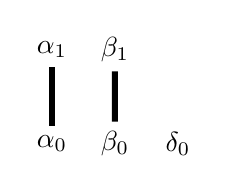
\begin{tikzpicture}[scale=0.4]
			\node (A0) at (0,0) {\textcolor{black}{$\alpha_0$}};
			\node (A1) at (0,3) {\textcolor{black}{$\alpha_1$}};
			\node (B0) at (2,0) {\textcolor{black}{$\beta_0$}};
			\node (B1) at (2,3) {\textcolor{black}{$\beta_1$}};
			\node (C0) at (4,0) {\textcolor{black}{$\delta_0$}};
			\draw[line width=.03in] (A0) -- (A1);
			\draw[line width=.03in] (B0) -- (B1);
		\end{tikzpicture} && 
		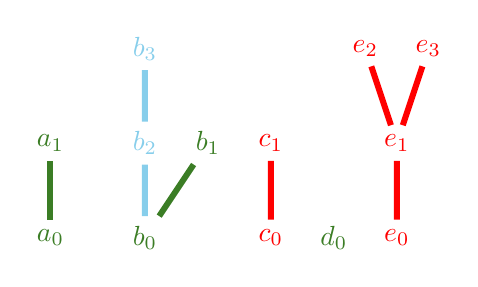
\begin{tikzpicture}[scale=0.4]
		\node (A0) at (0,0) {\textcolor{OliveGreen}{$a_0$}};
		\node (A1) at (0,3) {\textcolor{OliveGreen}{$a_1$}};
		\node (B0) at (3,0) {\textcolor{OliveGreen}{$b_0$}};
		\node (B1) at (3,3) {\textcolor{SkyBlue}{$b_2$}};
		\node (B2) at (5,3) {\textcolor{OliveGreen}{$b_1$}};
		\node (B3) at (3,6) {\textcolor{SkyBlue}{$b_3$}};
		\node (C0) at (7,0) {\textcolor{red}{$c_0$}};
		\node (C1) at (7,3) {\textcolor{red}{$c_1$}};
		\node (D0) at (9,0) {\textcolor{OliveGreen}{$d_0$}};
		\node (E0) at (11,0) {\textcolor{red}{$e_0$}};
		\node (E1) at (11,3) {\textcolor{red}{$e_1$}};
		\node (E2) at (10,6) {\textcolor{red}{$e_2$}};
		\node (E3) at (12,6) {\textcolor{red}{$e_3$}};
		
		\draw[OliveGreen, line width=.03in] (A0) -- (A1);
		\draw[SkyBlue,line width=.03in] (B0) -- (B1);
		\draw[OliveGreen,line width=.03in] (B0) -- (B2);
		\draw[SkyBlue, line width=.03in] (B1) -- (B3);
		\draw[red, line width=.03in] (C0) -- (C1);
		\draw[red, line width=.03in] (E0) -- (E1);
		\draw[red, line width=.03in] (E1) -- (E2);
		\draw[red, line width=.03in] (E1) -- (E3);
	\end{tikzpicture} \\
		& {{}} \\
		\textcolor{OliveGreen}{\bullet} && 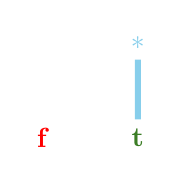
\begin{tikzpicture}[scale=0.4]
			\node (A) at (0,0) {\textcolor{red}{\textbf{f}}};
			\node (B) at (3,0) {\textcolor{OliveGreen}{\textbf{t}}};
			\node (C) at (3,3) {\textcolor{SkyBlue}{$*$}};
			\draw[SkyBlue, line width=.03in] (B) -- (C);
		\end{tikzpicture}
		\arrow["{\chi_f}"', from=1-3, to=3-3]
		\arrow["{!_F}", dashed, from=1-1, to=3-1]
		\arrow["true", from=3-1, to=3-3]
		\arrow[draw=none, from=1-1, to=2-2]
		\arrow["f"', tail, from=1-1, to=1-3]
		\arrow[draw=none, from=1-1, to=2-2]
		\arrow[ from=1-1, to=2-2, phantom, "\scalebox{1.5}{$\lrcorner$}",  very near start, color=black]
	\end{tikzcd}
\caption{Characteristic diagram of $f: F \hookrightarrow G$. }	
\end{figure}

Notice that $\chi_f$ assigns the value \textcolor{OliveGreen}{\textbf{t}} to the nodes of the sub-forest $f[F]$,  the value \textcolor{SkyBlue}{\textbf{$*$}} to any node that is not in the sub-forest but is in the up-set of $f(F)$ so  and the value \textcolor{red}{\textbf{f}} to any node that is not in the sub-forest nor in its up-set. 

\newpage
\subsection{Exponentials}

We now come to \emph{exponentiation}.

Recall what it means for a category $\mathbb{C}$ to have an \emph{exponential object}:
\begin{definition}[exponential objects]
	$\forall A, B \in \mathbb{C}$ there exists an exponential object $B^A \in \mathbb{C}$ and a map $eval : B^A \times A \rightarrow B$ such that the  \emph{universal mapping property} or UMP holds: For any $g :C \times A \rightarrow B$ there is a unique $\hat{g} :C \rightarrow B^A$ making the following diagram commute:
	
	\begin{figure}[h]
		\centering
		\begin{tikzcd}
			{B^A \times A} && B \\
			\\
			{C \times A}
			\arrow["g"', from=3-1, to=1-3]
			\arrow["{\hat{g}\times id_A}"', from=3-1, to=1-1]
			\arrow["eval"', from=1-1, to=1-3]
		\end{tikzcd}
		\caption{UMP}
	\end{figure}
	
\end{definition}

 \begin{remark}
 	The UMP can also be read as: $\forall g :C \times A \rightarrow B\;$ $\exists! \;\hat{g} :C \rightarrow B^A$ called an \emph{encoding of g} such that $eval \circ (\hat{g}\times id_A) = g$.
 \end{remark}


\begin{remark}
	This can also be seen as an \emph{adjunction} $ (-) \times A \dashv (-)^{A} $ between the \emph{product} and \emph{exponent} functors by a fixed object $A$ which gives rise to a 1:1 correspondence for any object $B$:
	\begin{gather*}
		Hom(C \times A, B) \cong Hom(C,B^A) \\
		g \xleftrightarrow{1:1} \hat{g}
	\end{gather*} 
\end{remark}
 
 Remember also that for finite sets $\mathbb{Set}_{fin}$  the exponential is defined as  $B^A := \{f : A \rightarrow B\}$ i.e., the set of functions from $A$ to $B$. \newline
 $\hat{g}$ is the result of the operation of \emph{currying} i.e., $\hat{g}(c) := g(c,-) : A \rightarrow B$ and \emph{eval} is \emph{evaluation} of a function $f$ in $a$ is $eval(f,a) := f(a)$ so that $eval \circ (\hat{g}\times id_A)(c,a) = eval(\hat{g}(c),a)=(\hat{g}(c))(a)=g(c,a)$.\newline
 \newline
 We now proceed outlining the steps used in \cite{towards}:\newline
 \newline
 Do exponential objects exist in $\mathbb{FF}_*$? \newline
 
 \emph{If} they exist then, since $\mathbb{FF}_*$ is a \emph{distributive} category:
 \begin{lem}
 	For all objects $ F,G,H $ in $\mathbb{FF}_* :$
 	\[ F^{(G+H)} \cong F^G \times F^H \]
 \end{lem}

Recall that any $F \in \mathbb{FF}_*$ can be written as $F= \sum_{i=1}^{N} T_i $ for some trees $\{T_i\}_{i=1}^N$, this allows us to reduce the study of the existence of exponentiation to the case $F^T$ for some tree $T$.\newline

Since $ C \cong (C \times 1) \rightarrow F$ is adjoint to $ C \rightarrow F^1 $ for any $C \in \mathbb{FF}_*$, we have $F^1 \cong F$ for every $F \in \mathbb{FF}_*$.
We now have:
\begin{remark}
	$\forall F,G \in \mathbb{FF}_* : (F+G)^1 \cong F^1 + G^1$.
\end{remark}
This can be generalized.
It can be shown that $F^T + G^T$ \emph{behaves as} $(F+G)^T$. \footnote{i.e., for each $f: H \times T \rightarrow F + G$ there is a unique $\hat{f}: H \rightarrow F^T + G^T$ such that $(e_F + e_G)\circ(\hat{f} \times id_T)=f$ with $e_F,e_G$ the evaluation maps for $F^T$ and $G^T$.}
\newline
What this entails is:
\begin{lem}$\forall F,G \in \mathbb{FF}_*, T \in \mathbb{T} :$
	\[ (F+G)^T \cong F^T + G^T\]
\end{lem}

In fact reducing further the study to the existence of the exponential $T^S$ for both $T,S \in \mathbb{T}$,
we now have for $F,G \in \mathbb{FF}_*$:
\begin{thm}
	For $ F = \sum_{i=1}^{n} T_i $ and $ G = \sum_{j=1}^{m} S_j :$
	\[ F^G \cong \prod_{j=1}^{m} \sum_{i=1}^{n} (T_i^{S_j}) \] 
\end{thm}

\newpage

Exponentiation for $\mathbb{FF}_1$ has been settled as $\mathbb{FF}_1 \simeq Set_{fin}$. \newline
The next "level up" is $\mathbb{FF}_2$ or the category of \emph{Bushes}. \newline
Each \emph{bush} in $\mathbb{FF}_2 \cap \mathbb{T}$ is of the form $B_\bot$ where $B$ is a finite anti-chain i.e., a finite set. \newline

By the previous considerations, we arrive at the main result of \cite{towards}: \newline
(Note that $ |A_\bot|$ denotes the cardinality of the underlying poset and $n\textbf{F}$ is shorthand for the n-th co-power of $\textbf{F}$).
\begin{thm}[\emph{bushes} have exponential objects]\label{thm:bushesexp}
 The following formula holds for all $A_\bot$ and $B_\bot$ $\in \mathbb{FF}_2 \cap \mathbb{T}$ :
\begin{equation}\label{exponent}
	B_\bot ^{A_\bot} \cong | B_\bot |^{|A|} (\;(\; (|B_\bot|^{|A_\bot|} -1)\mathbf{1} )_\bot\;)
\end{equation}

Using distributivity we can generalize this formula to arbitrary Bushes $F$ and $G$, written as sums of trees in $\mathbb{FF}_2$, $F=\sum_{i=1}^{m}(F_i)_\bot$ and $G=\sum_{j=1}^{n}(G_j)_\bot$:
\begin{equation}
	F ^ G \cong \prod_{j=1}^{n} \sum_{i=1}^{m} ( | (F_i)_\bot |^{|G_j|} (\;(\; (|(F_i)_\bot|^{|(G_j)_\bot|} -1)\mathbf{1} )_\bot\;) )
\end{equation}
\end{thm} 

 The intuition behind this fact is that trees in $\mathbb{FF}_2$ behave with respect to arrows nearly as finite sets. This is because arrows $f$ from $B_\bot$ to a target $C_\bot$ are  basically (Set-)functions with the only constraint that the root of $B_\bot$  be sent to the root of $C_\bot$.\newline
 
 Putting together the results in Theorem~\ref{thm:bushesexp},Corollary~\ref{cor:subobjcl} \& Lemma~\ref{lem:ffcomplete} we obtain:
 \begin{cor}[\emph{bushes} form a topos]
 	$\mathbb{FF}_2$/\emph{bushes} is an elementary topos.
 \end{cor}
 
 	We wrap up by giving a few examples of exponentials for Bushes:
 
 \begin{ex}
 	\begin{gather*}
 		\Omega^{\textbf{1}_\bot} \cong \textbf{1} + 2(3 \cdot \textbf{1})_\bot. \\
 		(\textbf{1}_\bot) ^{\Omega} \cong 2(7 \cdot \textbf{1})_\bot. \\
 		 \Omega^{\Omega} \cong \textbf{1} + \textbf{1}_\bot + 2(3 \cdot \textbf{1})_\bot + 2(7 \cdot \textbf{1})_\bot.  
 	\end{gather*}
 \end{ex}
 
 
\newpage
\subsection{\hl{An Exponential Example}}

 Let us examine how these exponential objects work with the example of arrows from $\textbf{1}_\bot \times \textbf{1}_\bot$ to $\textbf{1}_\bot$. \newline
 The formula \ref{exponent} says that the exponential object should be:
 \[ (\textbf{1}_\bot) ^ {\textbf{1}_\bot} \cong 2^1 ( ( (2^2-1)\textbf{1} )_\bot ) = 2( 3\cdot\textbf{1})_\bot \]

The universal mapping property (UMP) applied to this case states that the following diagram should commute.

\begin{figure}[h]
	\centering
	\begin{tikzcd}[scale=0.5]
		{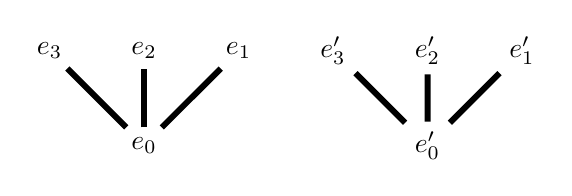
\begin{tikzpicture}[scale=0.4]
				\node (A) at (0,0) {$e_0$};
				\node (B) at (-3,3) {$e_3$};
				\node (C) at (0,3) {$e_2$};
				\node (D) at (3,3) {$e_1$};
				\draw[line width=.03in] (A) -- (B);
				\draw[line width=.03in] (A) -- (C);
				\draw[line width=.03in] (A) -- (D);
				
				\node (A') at (9,0) {$e_0'$};
				\node (B') at (6,3) {$e_3'$};
				\node (C') at (9,3) {$e_2'$};
				\node (D') at (12,3) {$e_1'$};
				\draw[line width=.03in] (A') -- (B');
				\draw[line width=.03in] (A') -- (C');
				\draw[line width=.03in] (A') -- (D');
			\end{tikzpicture} \times 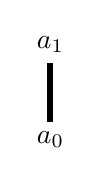
\begin{tikzpicture}[scale=0.4]
			\node (A) at (0,0) {$a_0$};
			\node (B) at (0,3) {$a_1$};
			
			\draw[line width=.03in] (A) -- (B);
			
		\end{tikzpicture}} && 
	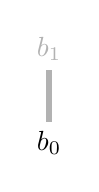
\begin{tikzpicture}[scale=0.4]
	\node (A) at (0,0) {$b_0$};
	\node (B) at (0,3) {\textcolor{gray!60}{$b_1$}};

	\draw[gray!60, line width=.03in] (A) -- (B);

	\end{tikzpicture} \\
		\\
		{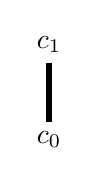
\begin{tikzpicture}[scale=0.4]
				\node (A) at (0,0) {$c_0$};
				\node (B) at (0,3) {$c_1$};
				
				\draw[line width=.03in] (A) -- (B);
				
			\end{tikzpicture} \times 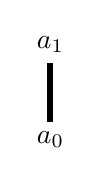
\begin{tikzpicture}[scale=0.4]
			\node (A) at (0,0) {$a_0$};
			\node (B) at (0,3) {$a_1$};
			
			\draw[line width=.03in] (A) -- (B);
			
		\end{tikzpicture}}
		\arrow["g"', from=3-1, to=1-3]
		\arrow["{\hat{g}\times id_A}"', from=3-1, to=1-1]
		\arrow["eval"', from=1-1, to=1-3]
	\end{tikzcd}
	\caption{UMP diagram for $A=B=C=\textbf{1}_\bot$. 	(Bushes)}
\end{figure}

To understand how to construct the \emph{adjoint} arrow $\hat{g} : \textbf{1}_\bot \rightarrow (\textbf{1}_\bot)^{\textbf{1}_\bot} $ of $g : \textbf{1}_\bot \times \textbf{1}_\bot \rightarrow \textbf{1}_\bot$ let us take a look at all the possible maps (black dots are mapped to the root $b_0$ of $B=\textbf{1}_\bot$ whilst gray dots to $b_1$):
\newline
For example, one of these maps $g_1$ is:
\begin{figure}[h]
	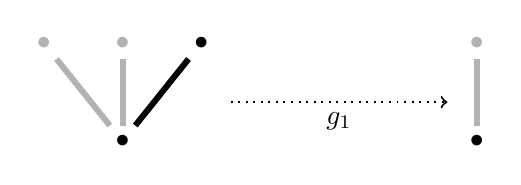
\begin{tikzpicture}[scale=0.25]
		
		\node (A) at (0,0) {$\textcolor{black}{\bullet}$};
		\node (B) at (-4,5) {$\textcolor{gray!60}{\bullet}$};
		\node (C) at (0,5) {$\textcolor{gray!60}{\bullet}$};
		\node (D) at (4,5) {$\textcolor{black}{\bullet}$};
		\node (d) at (5,2) {};
		
		\draw[gray!60, line width=.03in] (A) -- (B);
		\draw[gray!60, line width=.03in] (A) -- (C);
		\draw[line width=.03in] (A) -- (D);
		
		\node (e) at (17,2) {};
		\node (E) at (18,0) {$\textcolor{black}{\bullet}$};
		\node (F) at (18,5) {$\textcolor{gray!60}{\bullet}$};
		\draw[gray!60, line width=.03in] (E) -- (F);
		
		\draw[->, dotted, line width=.01in] (d) -- node[anchor=north] {$g_1$} (e);
	\end{tikzpicture}
	\caption{$C \times A = \textbf{1}_\bot \times \textbf{1}_\bot$ is displayed on the left and $B = \textbf{1}_\bot$ on the right. The map $g_1$ sends the nodes on the left object to nodes with matching color on the right object.}	
\end{figure}

%\begin{figure}[h]
%	\begin{tikzpicture}[scale=0.25]
%		
%		\node (A) at (0,0) {$\bot$};
%		\node (B) at (0,5) {$\textcolor{orange}{\bullet}$};
%		\node (d) at (1,2) {};
%		
%		\draw[orange, line width=.03in] (A) -- (B);
%		
%		\node (e) at (10,2) {};
%		
%		\node (E) at (12,0) {$e_0$};
%		\node (F) at (9,5) {$e_3$};
%		\node (G) at (12,5) {$e_2$};
%		\node (H) at (15,5) {$\textcolor{orange}{e_1}$};
%		\draw[line width=.03in] (E) -- (F);
%		\draw[line width=.03in] (E) -- (G);
%		\draw[orange, line width=.03in] (E) -- (H);
%		
%		\node (E') at (22,0) {$e_7$};
%		\node (F') at (19,5) {$e_6$};
%		\node (G') at (22,5) {$e_5$};
%		\node (H') at (25,5) {$e_4$};
%		\draw[line width=.03in] (E') -- (F');
%		\draw[line width=.03in] (E') -- (G');
%		\draw[line width=.03in] (E') -- (H');
%		
%		\draw[->, dotted, line width=.01in] (d) -- node[anchor=north] {$\hat{g_1}$} (e);
%	\end{tikzpicture}
%	\caption{}
%	\end{figure}




\begin{figure}[h]
	\centering
	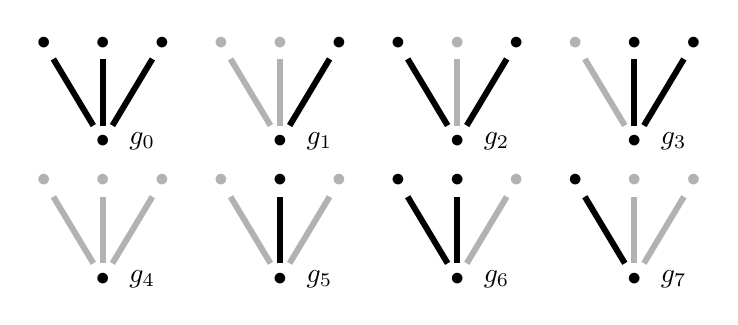
\begin{tikzpicture}[scale=0.25]
		\node (A) at (0,0) {$\textcolor{black}{\bullet} $};
		\node (N) at (2,0) {$g_0$};
		\node (B) at (-3,5) {$\textcolor{black}{\bullet}$};
		\node (C) at (0,5) {$\textcolor{black}{\bullet}$};
		\node (D) at (3,5) {$\textcolor{black}{\bullet}$};
		\draw[line width=.03in] (A) -- (B);
		\draw[line width=.03in] (A) -- (C);
		\draw[line width=.03in] (A) -- (D);
		
		\node (A') at (9,0) {$\textcolor{black}{\bullet}$};
		\node (N') at (11,0) {$g_1$};
		\node (B') at (6,5) {$\textcolor{gray!60}{\bullet}$};
		\node (C') at (9,5) {$\textcolor{gray!60}{\bullet}$};
		\node (D') at (12,5) {$\textcolor{black}{\bullet}$};
		\draw[gray!60, line width=.03in] (A') -- (B');
		\draw[gray!60, line width=.03in] (A') -- (C');
		\draw[line width=.03in] (A') -- (D');
		
		\node (A'') at (18,0) {$\textcolor{black}{\bullet}$};
		\node (N'') at (20,0) {$g_2$};
		\node (B'') at (15,5) {$\textcolor{black}{\bullet}$};
		\node (C'') at (18,5) {$\textcolor{gray!60}{\bullet}$};
		\node (D'') at (21,5) {$\textcolor{black}{\bullet}$};
		\draw[line width=.03in] (A'') -- (B'');
		\draw[gray!60,line width=.03in] (A'') -- (C'');
		\draw[line width=.03in] (A'') -- (D'');
	
		\node (A''') at (27,0) {$\textcolor{black}{\bullet}$};
		\node (N''') at (29,0) {$g_3$};
		\node (B''') at (24,5) {$\textcolor{gray!60}{\bullet}$};
		\node (C''') at (27,5) {$\textcolor{black}{\bullet}$};
		\node (D''') at (30,5) {$\textcolor{black}{\bullet}$};
		\draw[gray!60,line width=.03in] (A''') -- (B''');
		\draw[line width=.03in] (A''') -- (C''');
		\draw[line width=.03in] (A''') -- (D''');
		
		\node (A'''') at (0,-7) {$\textcolor{black}{\bullet}$};
		\node (N'''') at (2,-7) {$g_4$};
		\node (B'''') at (-3,-2) {$\textcolor{gray!60}{\bullet}$};
		\node (C'''') at (0,-2) {$\textcolor{gray!60}{\bullet}$};
		\node (D'''') at (3,-2) {$\textcolor{gray!60}{\bullet}$};
		\draw[gray!60, line width=.03in] (A'''') -- (B'''');
		\draw[gray!60, line width=.03in] (A'''') -- (C'''');
		\draw[gray!60, line width=.03in] (A'''') -- (D'''');
		
		\node (A''''') at (9,-7) {$\textcolor{black}{\bullet}$};
		\node (N''''') at (11,-7) {$g_5$};
		\node (B''''') at (6,-2) {$\textcolor{gray!60}{\bullet}$};
		\node (C''''') at (9,-2) {$\textcolor{black}{\bullet}$};
		\node (D''''') at (12,-2) {$\textcolor{gray!60}{\bullet}$};
		\draw[gray!60, line width=.03in] (A''''') -- (B''''');
		\draw[line width=.03in] (A''''') -- (C''''');
		\draw[gray!60, line width=.03in] (A''''') -- (D''''');
		
		\node (A'''''') at (18,-7) {$\textcolor{black}{\bullet}$};
		\node (N'''''') at (20,-7) {$g_6$};
		\node (B'''''') at (15,-2) {$\textcolor{black}{\bullet}$};
		\node (C'''''') at (18,-2) {$\textcolor{black}{\bullet}$};
		\node (D'''''') at (21,-2) {$\textcolor{gray!60}{\bullet}$};
		\draw[line width=.03in] (A'''''') -- (B'''''');
		\draw[ line width=.03in] (A'''''') -- (C'''''');
		\draw[gray!60, line width=.03in] (A'''''') -- (D'''''');
		
		\node (A''''''') at (27,-7) {$\textcolor{black}{\bullet}$};
		\node (N''''''') at (29,-7) {$g_7$};
		\node (B''''''') at (24,-2) {$\textcolor{black}{\bullet}$};
		\node (C''''''') at (27,-2) {$\textcolor{gray!60}{\bullet}$};
		\node (D''''''') at (30,-2) {$\textcolor{gray!60}{\bullet}$};
		\draw[line width=.03in] (A''''''') -- (B''''''');
		\draw[gray!60, line width=.03in] (A''''''') -- (C''''''');
		\draw[gray!60, line width=.03in] (A''''''') -- (D''''''');
\end{tikzpicture}
	\caption{All the possible maps $g_j : \textbf{1}_\bot \times \textbf{1}_\bot \rightarrow \textbf{1}_\bot$ for j=0,..,7. 	(Bushes)}
\end{figure}

Notice that:
\begin{lem}
	$|Hom(\textbf{1}_\bot \times \textbf{1}_\bot, \textbf{1}_\bot)|=8$.
\end{lem}
  This result could be computed by simply counting the number of distinct set-functions from $3\cdot \textbf{1}$ to $\textbf{1}_\bot$ which is $2^3$ since as we saw $\textbf{1}_\bot \times \textbf{1}_\bot = (3\cdot \textbf{1})_\bot$ and there are no constraints on where the non-root elements are assigned. \newline

How to obtain the adjoint maps $\hat{g}_j$?\newline

The \emph{product map} $\hat{g}_j \times id_A$ by definition must satisfy:
\begin{enumerate}
	\item $\pi_{B^A}\circ(\hat{g}_j \times id_A) = \hat{g}_j$.
	\item $\pi_{A}\circ(\hat{g}_j \times id_A) = id_A$.
\end{enumerate}
From the first condition, the fibers for $i=0,1$ $\pi_C^{-1}\{c_i\}$ of $C \times A$ must be mapped to the corresponding fibers of $\pi_{B^A}^{-1}\{\hat{g}_j(c_i)\}$ of $B^A \times A$. \newline
From the second condition, the fibers for $i=0,1$ $\pi_A^{-1}\{a_i\}$ of $C \times A$ must be mapped to the corresponding fibers of $\pi_A^{-1}\{a_i\}$ of $B^A \times A$. \newline

The \emph{eval} map can now be constructed on the product $B^A \times A$.


\begin{figure}[h]
	\begin{tikzcd}
		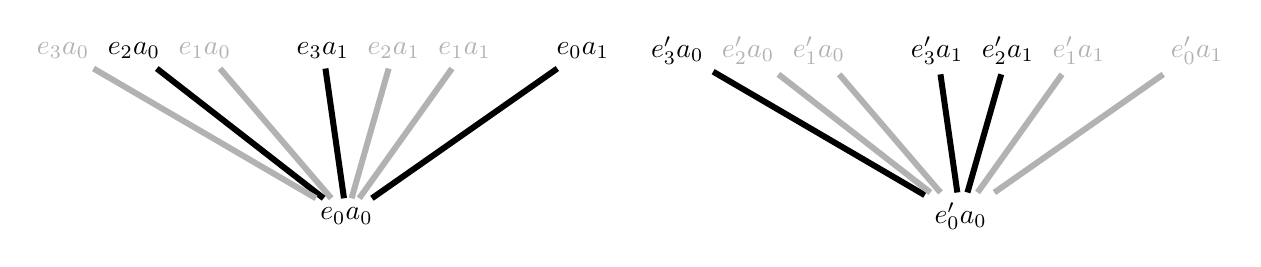
\begin{tikzpicture}[scale=0.3]
			\node (H) at (-22,3) {\textcolor{gray!60}{$e_3 a_0$}};
			\node (G) at (-19,3) {$e_2 a_0$};
			\node (F) at (-16,3) {\textcolor{gray!60}{$e_1 a_0$}};
			\node (A) at (-10,-4) {$e_0 a_0$};
			\node (B) at (-11,3) {$e_3 a_1$};
			\node (C) at (-8,3) {\textcolor{gray!60}{$e_2 a_1$}};
			\node (D) at (-5,3) {\textcolor{gray!60}{$e_1 a_1$}};
			\node (E) at (0,3) {$e_0 a_1$};
			
			\draw[line width=.03in] (A) -- (B);
			\draw[gray!60, line width=.03in] (A) -- (C);
			\draw[gray!60, line width=.03in] (A) -- (D);
			\draw[line width=.03in] (A) -- (E);
			\draw[gray!60, line width=.03in] (A) -- (F);
			\draw[line width=.03in] (A) -- (G);
			\draw[gray!60, line width=.03in] (A) -- (H);
			
			\node (H') at (4,3) {$e_3' a_0$};
			\node (G') at (7,3) {\textcolor{gray!60}{$e_2' a_0$}};
			\node (F') at (10,3) {\textcolor{gray!60}{$e_1' a_0$}};
			\node (A') at (16,-4) {$e_0'a_0$};
			\node (B') at (15,3) {$e_3'a_1$};
			\node (C') at (18,3) {$e_2'a_1$};
			\node (D') at (21,3) {\textcolor{gray!60}{$e_1' a_1$}};
			\node (E') at (26,3) {\textcolor{gray!60}{$e_0' a_1$}};
			
			\draw[line width=.03in] (A') -- (H');
			\draw[gray!60, line width=.03in] (A') -- (G');
			\draw[gray!60, line width=.03in] (A') -- (F');
			\draw[line width=.03in] (A') -- (B');
			\draw[line width=.03in] (A') -- (C');
			\draw[gray!60, line width=.03in] (A') -- (D');
			\draw[gray!60, line width=.03in] (A') -- (E');
			
			
		\end{tikzpicture} \\
		\\
		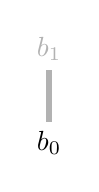
\begin{tikzpicture}[scale=0.3]
			\node (A) at (0,0) {$b_0$};
			\node (B) at (0,4) {\textcolor{gray!60}{$b_1$}};
			
			\draw[gray!60, line width=.03in] (A) -- (B);
			
		\end{tikzpicture}
		\arrow["eval"', from=1-1, to=3-1]
	\end{tikzcd}
	\caption{The map $eval : (\textbf{1}_\bot)^{\textbf{1}_\bot}\times \textbf{1}_\bot \rightarrow \textbf{1}_\bot$. 
		%(The pre-image of the root $b_0$ is displayed in black and that of $b_1$ in gray)
			(Bushes) \newline (The usual labeling notation on nodes is used for product objects whereby the left and right letters specify the left and right projections respectively). 
	}
\end{figure}

Starting off from the map $g_0$ which sends every node to the root $b_0$ we have that $\hat{g}_0 : C=\textbf{1}_\bot \rightarrow \textbf{1}_\bot^{\textbf{1}_\bot}$ must send the nodes $c_0$ and $c_1$ of $C$ to a root (either $e_0$ or $e_0'$) of one of the trees $T_1$($\cong (3\cdot\textbf{1})_\bot$) or $T_2$ ($\cong (3\cdot\textbf{1})_\bot$). \newline

Without loss of generality we can say that $\hat{g}_0$ maps $c_0,c_1$ to the root $e_0$ of $T_1$. \newline
By a similar argument we find that $\hat{g}_1 :c_0 \mapsto e_0$ \footnote{recall that every root must be mapped to a root.} and $c_1 \mapsto e_1$. \newline
Also $\hat{g}_2 : c_0 \mapsto e_0, c_1 \mapsto e_2$ and $\hat{g}_3 : c_0 \mapsto e_0, c_1 \mapsto e_3$.   
The rest follow in a similar fashion with the maps $\hat{g}_k$ $k=4,..,7$ sending $c_0$ to $e_0'$ instead.\newline
By requiring that the UMP diagram commute, the fibers for $j=0,..,7$ of $g_j^{-1}\{b_i\}$ for $i=0,1$ must be preserved by the mapping $\hat{g}_j \times id_A$ .
\newpage
Note that $\hat{g}_j$ is entirely determined by $\hat{g}_j(c_1)$ since we know that $c_0$ maps to the root of the tree that contains $\hat{g}_j(c_1)$.
This suggests the following:
\begin{lem}
	The exponential object $(\textbf{1}_\bot) ^ {\textbf{1}_\bot}$ \emph{encodes} the maps $\{g_j\}_{j=0}^7$.
\end{lem}
%check
It is worth pausing here and make a more general categorical consideration which will come in useful later on:
 \begin{prop}\label{representing}
 	In $\mathbb{FF_2}$/\emph{bushes} we have that $\textbf{1}_\bot$ is the representing object i.e., 
 	\[ \mathbb{FF_2}(\textbf{1}_\bot, F) \cong |F| \]
 	whereby $|F|$ denotes the underlying set of the finite forest $F$.
 \end{prop}
 \begin{proof}
 	Let $\textbf{1}_\bot = \{ \bot < \bullet\}$ and $|F| = \{a_j\}_{j=1}^n$ where each $a_j$ is either
 	a root $r_j$ or on top of (a unique) one i.e., $r_j < a_j$. \newline
 	The bijection is realized as we saw earlier by $f_j \leftrightarrow a_j$ where:
 	\[f_j := \bullet \mapsto a_j \;\;\text{ and } \bot \mapsto r_j\]
 \end{proof}
 
 
We resume our example: \newline
  This \emph{encoding} can be visualized by labeling each node that corresponds to $\hat{g}_j(c_1)$ with the map $g_j$ so that the following figure is obtained:

\begin{figure}[h]
	\centering
	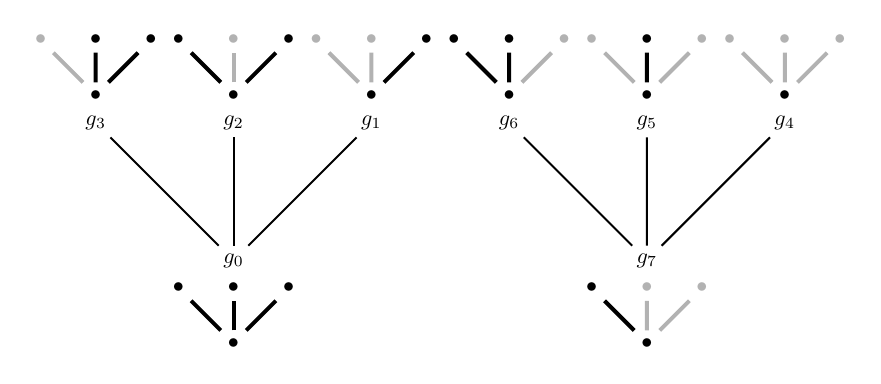
\begin{tikzpicture}[scale=0.35, every node/.style={scale=0.8}]
		\node (A) at (0,0) {$g_0$};
			\node (C0) at (0,-1) {\textcolor{black}{$\bullet$}};
			\node (B0) at (-2,-1) {\textcolor{black}{$\bullet$}};
			\node (D0) at (2,-1) {\textcolor{black}{$\bullet$}};
			\node (A0) at (0,-3) {\textcolor{black}{$\bullet$}};
			\draw[line width=.02in] (A0) -- (B0);
			\draw[line width=.02in] (A0) -- (C0);
			\draw[line width=.02in] (A0) -- (D0);
		\node (B) at (-5,5) {$g_3$};
			\node (C3) at (-5,8) {\textcolor{black}{$\bullet$}};
			\node (B3) at (-7,8) {\textcolor{gray!60}{$\bullet$}};
			\node (D3) at (-3,8) {\textcolor{black}{$\bullet$}};
			\node (A3) at (-5,6) {\textcolor{black}{$\bullet$}};
			\draw[gray!60, line width=.02in] (A3) -- (B3);
			\draw[line width=.02in] (A3) -- (C3);
			\draw[line width=.02in] (A3) -- (D3);
		\node (C) at (0,5) {$g_2$};
			\node (C2) at (0,8) {\textcolor{gray!60}{$\bullet$}};
			\node (B2) at (-2,8) {\textcolor{black}{$\bullet$}};
			\node (D2) at (2,8) {\textcolor{black}{$\bullet$}};
			\node (A2) at (0,6) {\textcolor{black}{$\bullet$}};
			\draw[line width=.02in] (A2) -- (B2);
			\draw[gray!60, line width=.02in] (A2) -- (C2);
			\draw[line width=.02in] (A2) -- (D2);
		\node (D) at (5,5) {$g_1$};
			\node (C1) at (5,8) {\textcolor{gray!60}{$\bullet$}};
			\node (B1) at (3,8) {\textcolor{gray!60}{$\bullet$}};
			\node (D1) at (7,8) {\textcolor{black}{$\bullet$}};
			\node (A1) at (5,6) {\textcolor{black}{$\bullet$}};
			\draw[gray!60, line width=.02in] (A1) -- (B1);
			\draw[gray!60, line width=.02in] (A1) -- (C1);
			\draw[line width=.02in] (A1) -- (D1);
			
		\draw[line width=.01in] (A) -- (B);
		\draw[line width=.01in] (A) -- (C);
		\draw[line width=.01in] (A) -- (D);
		
		\node (A') at (15,0) {$g_7$};
			\node (C0') at (15,-1) {\textcolor{gray!60}{$\bullet$}};
			\node (B0') at (13,-1) {\textcolor{black}{$\bullet$}};
			\node (D0') at (17,-1) {\textcolor{gray!60}{$\bullet$}};
			\node (A0') at (15,-3) {\textcolor{black}{$\bullet$}};
			\draw[line width=.02in] (A0') -- (B0');
			\draw[gray!60, line width=.02in] (A0') -- (C0');
			\draw[gray!60, line width=.02in] (A0') -- (D0');
		\node (B') at (10,5) {$g_6$};
			\node (C1') at (10,8) {\textcolor{black}{$\bullet$}};
			\node (B1') at (8,8) {\textcolor{black}{$\bullet$}};
			\node (D1') at (12,8) {\textcolor{gray!60}{$\bullet$}};
			\node (A1') at (10,6) {\textcolor{black}{$\bullet$}};
			\draw[ line width=.02in] (A1') -- (B1');
			\draw[ line width=.02in] (A1') -- (C1');
			\draw[gray!60, line width=.02in] (A1') -- (D1');		
		\node (C') at (15,5) {$g_5$};
			\node (C2') at (15,8) {\textcolor{black}{$\bullet$}};
			\node (B2') at (13,8) {\textcolor{gray!60}{$\bullet$}};
			\node (D2') at (17,8) {\textcolor{gray!60}{$\bullet$}};
			\node (A2') at (15,6) {\textcolor{black}{$\bullet$}};
			\draw[gray!60, line width=.02in] (A2') -- (B2');
			\draw[line width=.02in] (A2') -- (C2');
			\draw[gray!60, line width=.02in] (A2') -- (D2');		
		\node (D') at (20,5) {$g_4$};
			\node (C3') at (20,8) {\textcolor{gray!60}{$\bullet$}};
			\node (B3') at (18,8) {\textcolor{gray!60}{$\bullet$}};
			\node (D3') at (22,8) {\textcolor{gray!60}{$\bullet$}};
			\node (A3') at (20,6) {\textcolor{black}{$\bullet$}};
			\draw[gray!60, line width=.02in] (A3') -- (B3');
			\draw[gray!60, line width=.02in] (A3') -- (C3');
			\draw[gray!60, line width=.02in] (A3') -- (D3');
		\draw[line width=.01in] (A') -- (B');
		\draw[line width=.01in] (A') -- (C');
		\draw[line width=.01in] (A') -- (D');
	\end{tikzpicture}
	\caption{The encoded maps in $(\textbf{1}_\bot) ^ {\textbf{1}_\bot}$.	(Bushes)}
\end{figure}

The category of \emph{bushes} $\mathbb{FF}_2$ is a \emph{topos}.
\newline
What about \emph{higher} finite forests $\mathbb{FF}_k$ with $k\geq 3$ ?
\newline\newline
(Henceforth we denote $\mathbb{FF}_k$ with $k\geq 3$ by $\mathbb{FF}_{k\geq3}$.)



\newpage
\section{When Forests fail to be a Topos} 
\label{counterex}

As the title suggests in this section we are going to prove that finite forests $\mathbb{FF}_k$ higher than bushes with $k>2$ \emph{fail} to be a topos by detailing step by step a novel constructive counter-example. \newline\newline
The failure occurs when we require the existence of exponential objects.
Recall that exponentiation for Bushes was obtained thanks to the fact that every tree in $\mathbb{FF}_2$ was of the form $F_\bot$ with $F$ a finite anti-chain or set. Thus every map between trees $B_\bot \rightarrow C_\bot$ was essentially a set-function with the only requirement that the root node be mapped to the root of the target. This property is lost when we move to $\mathbb{FF}_k$ with $k>2$. \newline
In fact, as we shall prove: $\mathbb{FF}_k$ with $k>2$ generally fails to have exponential objects.
\newpage
\subsection{\hl{Counter-example for $\mathbb{FF}_3$}}

Let's start by re-examining the previous example of $g: \textbf{1}_\bot \times \textbf{1}_\bot \rightarrow \textbf{1}_\bot$. Though this time $\times$ is taken not to be $\times_{\mathbb{FF}_2}$ but rather $\times_{\mathbb{FF}}$. \newline
Let us take a look at some of the possible maps.

For example, one of these maps $g_1$ is:
\begin{figure}[h]
	\centering
	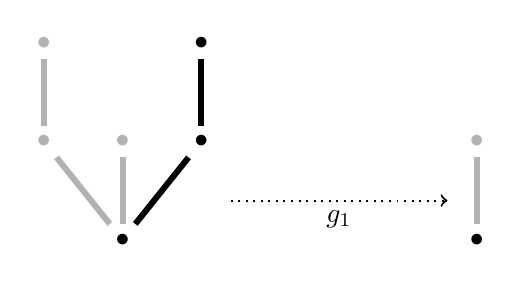
\begin{tikzpicture}[scale=0.25]
		
		\node (A) at (0,0) {$\textcolor{black}{\bullet}$};
		\node (B) at (-4,5) {$\textcolor{gray!60}{\bullet}$};
		\node (B') at (-4,10) {$\textcolor{gray!60}{\bullet}$};
		\node (C) at (0,5) {$\textcolor{gray!60}{\bullet}$};
		\node (D) at (4,5) {$\textcolor{black}{\bullet}$};
		\node (D') at (4,10) {$\textcolor{black}{\bullet}$};
		\node (d) at (5,2) {};
		
		\draw[gray!60, line width=.03in] (A) -- (B);
		\draw[gray!60, line width=.03in] (B) -- (B');
		\draw[gray!60, line width=.03in] (A) -- (C);
		\draw[line width=.03in] (A) -- (D);
		\draw[line width=.03in] (D) -- (D');
		
		\node (e) at (17,2) {};
		\node (E) at (18,0) {$\textcolor{black}{\bullet}$};
		\node (F) at (18,5) {$\textcolor{gray!60}{\bullet}$};
		\draw[gray!60, line width=.03in] (E) -- (F);
		
		\draw[->, dotted, line width=.01in] (d) -- node[anchor=north] {$g_1$} (e);
	\end{tikzpicture}
\caption{
	As before black dots are mapped to the root $b_0$ of $B=\textbf{1}_\bot$ whilst gray dots to $b_1$.}
\end{figure}


\begin{figure}[h]
	\centering
	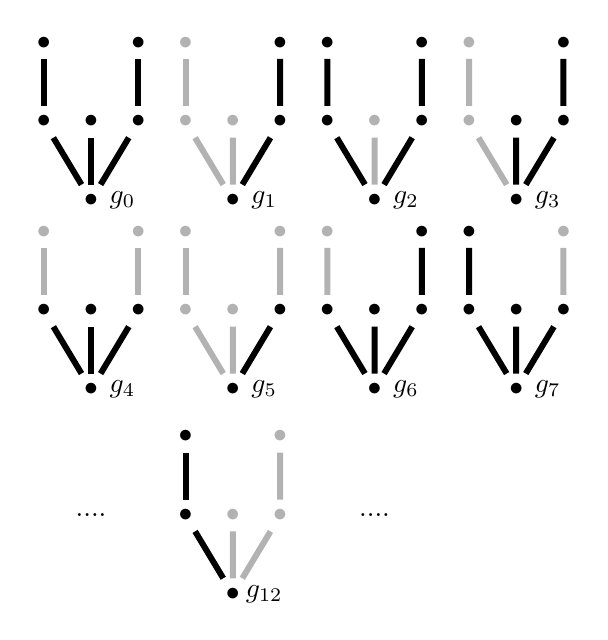
\begin{tikzpicture}[scale=0.2]
		\node (A) at (0,0) {$\textcolor{black}{\bullet} $};
		\node (N) at (2,0) {$g_0$};
			\node (B) at (-3,5) {$\textcolor{black}{\bullet}$};
				\node (E) at (-3,10) {$\textcolor{black}{\bullet}$};
			\node (C) at (0,5) {$\textcolor{black}{\bullet}$};
			\node (D) at (3,5) {$\textcolor{black}{\bullet}$};
				\node (F) at (3,10) {$\textcolor{black}{\bullet}$};
		\draw[line width=.03in] (A) -- (B);
			\draw[line width=.03in] (B) -- (E);
		\draw[line width=.03in] (A) -- (C);
		\draw[line width=.03in] (A) -- (D);
			\draw[line width=.03in] (D) -- (F);
		
		\node (A') at (9,0) {$\textcolor{black}{\bullet}$};
		\node (N') at (11,0) {$g_1$};
			\node (B') at (6,5) {$\textcolor{gray!60}{\bullet}$};
				\node (E') at (6,10) {$\textcolor{gray!60}{\bullet}$};
			\node (C') at (9,5) {$\textcolor{gray!60}{\bullet}$};
			\node (D') at (12,5) {$\textcolor{black}{\bullet}$};
				\node (F') at (12,10) {$\textcolor{black}{\bullet}$};
		\draw[gray!60, line width=.03in] (A') -- (B');
			\draw[gray!60, line width=.03in] (B') -- (E');
		\draw[gray!60, line width=.03in] (A') -- (C');
		\draw[line width=.03in] (A') -- (D');
			\draw[line width=.03in] (D') -- (F');
		
		\node (A'') at (18,0) {$\textcolor{black}{\bullet}$};
		\node (N'') at (20,0) {$g_2$};
			\node (B'') at (15,5) {$\textcolor{black}{\bullet}$};
				\node (E'') at (15,10) {$\textcolor{black}{\bullet}$};
			\node (C'') at (18,5) {$\textcolor{gray!60}{\bullet}$};
			\node (D'') at (21,5) {$\textcolor{black}{\bullet}$};
				\node (F'') at (21,10) {$\textcolor{black}{\bullet}$};
		\draw[line width=.03in] (A'') -- (B'');
			\draw[line width=.03in] (B'') -- (E'');
		\draw[gray!60,line width=.03in] (A'') -- (C'');
		\draw[line width=.03in] (A'') -- (D'');
			\draw[line width=.03in] (D'') -- (F'');
		
		\node (A''') at (27,0) {$\textcolor{black}{\bullet}$};
		\node (N''') at (29,0) {$g_3$};
			\node (B''') at (24,5) {$\textcolor{gray!60}{\bullet}$};
				\node (E''') at (24,10) {$\textcolor{gray!60}{\bullet}$};
			\node (C''') at (27,5) {$\textcolor{black}{\bullet}$};
			\node (D''') at (30,5) {$\textcolor{black}{\bullet}$};
				\node (F''') at (30,10) {$\textcolor{black}{\bullet}$};
			\draw[gray!60,line width=.03in] (A''') -- (B''');
				\draw[gray!60,line width=.03in] (B''') -- (E''');
			\draw[line width=.03in] (A''') -- (C''');
			\draw[line width=.03in] (A''') -- (D''');
				\draw[line width=.03in] (D''') -- (F''');
		
		\node (A'''') at (0,-12) {$\textcolor{black}{\bullet}$};
		\node (N'''') at (2,-12) {$g_4$};
			\node (B'''') at (-3,-7) {$\textcolor{black}{\bullet}$};
				\node (E'''') at (-3,-2) {$\textcolor{gray!60}{\bullet}$};
			\node (C'''') at (0,-7) {$\textcolor{black}{\bullet}$};
			\node (D'''') at (3,-7) {$\textcolor{black}{\bullet}$};
				\node (F'''') at (3,-2) {$\textcolor{gray!60}{\bullet}$};
			\draw[line width=.03in] (A'''') -- (B'''');
				\draw[gray!60, line width=.03in] (B'''') -- (E'''');
			\draw[line width=.03in] (A'''') -- (C'''');
			\draw[line width=.03in] (A'''') -- (D'''');
				\draw[gray!60, line width=.03in] (D'''') -- (F'''');
		
		\node (A''''') at (9,-12) {$\textcolor{black}{\bullet}$};
		\node (N''''') at (11,-12) {$g_5$};
			\node (B''''') at (6,-7) {$\textcolor{gray!60}{\bullet}$};
				\node (E''''') at (6,-2) {$\textcolor{gray!60}{\bullet}$};
			\node (C''''') at (9,-7) {$\textcolor{gray!60}{\bullet}$};
			\node (D''''') at (12,-7) {$\textcolor{black}{\bullet}$};
				\node (F''''') at (12,-2) {$\textcolor{gray!60}{\bullet}$};
			\draw[gray!60, line width=.03in] (A''''') -- (B''''');
				\draw[gray!60, line width=.03in] (B''''') -- (E''''');
			\draw[gray!60, line width=.03in] (A''''') -- (C''''');
			\draw[line width=.03in] (A''''') -- (D''''');
				\draw[gray!60, line width=.03in] (D''''') -- (F''''');
		
		\node (A'''''') at (18,-12) {$\textcolor{black}{\bullet}$};
		\node (N'''''') at (20,-12) {$g_6$};
			\node (B'''''') at (15,-7) {$\textcolor{black}{\bullet}$};
				\node (E'''''') at (15,-2) {$\textcolor{gray!60}{\bullet}$};
			\node (C'''''') at (18,-7) {$\textcolor{black}{\bullet}$};
			\node (D'''''') at (21,-7) {$\textcolor{black}{\bullet}$};
				\node (F'''''') at (21,-2) {$\textcolor{black}{\bullet}$};
		\draw[line width=.03in] (A'''''') -- (B'''''');
			\draw[gray!60, line width=.03in] (B'''''') -- (E'''''');
		\draw[ line width=.03in] (A'''''') -- (C'''''');
		\draw[line width=.03in] (A'''''') -- (D'''''');
			\draw[line width=.03in] (D'''''') -- (F'''''');
		
		\node (A''''''') at (27,-12) {$\textcolor{black}{\bullet}$};
		\node (N''''''') at (29,-12) {$g_7$};
			\node (B''''''') at (24,-7) {$\textcolor{black}{\bullet}$};
				\node (E''''''') at (24,-2) {$\textcolor{black}{\bullet}$};
			\node (C''''''') at (27,-7) {$\textcolor{black}{\bullet}$};
			\node (D''''''') at (30,-7) {$\textcolor{black}{\bullet}$};
				\node (F''''''') at (30,-2) {$\textcolor{gray!60}{\bullet}$};
			\draw[line width=.03in] (A''''''') -- (B''''''');
				\draw[line width=.03in] (B''''''') -- (E''''''');
			\draw[line width=.03in] (A''''''') -- (C''''''');
			\draw[line width=.03in] (A''''''') -- (D''''''');
				\draw[gray!60, line width=.03in] (D''''''') -- (F''''''');
				
		\node (n) at (0,-20) {....};
		
			\node (A0) at (9,-25) {$\textcolor{black}{\bullet}$};
			\node (N0) at (11,-25) {$g_{12}$};
				\node (B0) at (6,-20) {$\textcolor{black}{\bullet}$};
					\node (E0) at (6,-15) {$\textcolor{black}{\bullet}$};
				\node (C0) at (9,-20) {$\textcolor{gray!60}{\bullet}$};
				\node (D0) at (12,-20) {$\textcolor{gray!60}{\bullet}$};
					\node (F0) at (12,-15) {$\textcolor{gray!60}{\bullet}$};
				\draw[line width=.03in] (A0) -- (B0);
					\draw[line width=.03in] (B0) -- (E0);
				\draw[gray!60, line width=.03in] (A0) -- (C0);
				\draw[gray!60, line width=.03in] (A0) -- (D0);
					\draw[gray!60, line width=.03in] (D0) -- (F0);
					
	\node (n') at (18,-20) {....};
	\end{tikzpicture}
	\caption{The maps $g_j : \textbf{1}_\bot \times \textbf{1}_\bot \rightarrow \textbf{1}_\bot$ for $ j=0,..,17 $. }
\end{figure}

Notice that in this case:
\begin{lem}
	$|Hom(\textbf{1}_\bot \times \textbf{1}_\bot, \textbf{1}_\bot)|=18=|Hom(\textbf{1}_\bot, (\textbf{1}_\bot)^{\textbf{1}_\bot})|$.
\end{lem}
The previous result can be obtained in a number of ways. One of them is to count all the possible \emph{extensions} in $\mathbb{FF}$ of the old maps $g_j$ used in $\mathbb{FF}_2$. Another is to count all the possible sub-forests or down-sets of $\textbf{1}_\bot \times \textbf{1}_\bot$ since $B$ has only two elements and the pre-image of the root $b_0$ uniquely determines the map. \newline
The exponential object $(\textbf{1}_\bot)^{\textbf{1}_\bot}$ for $\mathbb{FF}_k$ $k>2$ is not readily given by some formula as in the case of Bushes. 
However, we have reason to state that in this case:
\begin{lem}\label{lem:superforest}
The \emph{candidate} for $(\textbf{1}_\bot)^{\textbf{1}_\bot}$ must be a \emph{super-forest} of the same-name exponential object found for the category of Bushes i.e., of $ 2(3 \cdot \textbf{1})_\bot $.
\end{lem}
This is due to the fact that $\textbf{1}_\bot \times_{\mathbb{FF}_2} \textbf{1}_\bot$ is by definition a sub-forest (of nodes of height at most 2) of $\textbf{1}_\bot \times_{\mathbb{FF}} \textbf{1}_\bot$ and the maps \emph{encoded} by $\textbf{1}_\bot \times_{\mathbb{FF}} \textbf{1}_\bot$ are all \emph{extensions} of maps already encoded by $\textbf{1}_\bot \times_{\mathbb{FF}_2} \textbf{1}_\bot$. 

\begin{remark}
	Another approach to Lemma~\ref{lem:superforest} is obtained by looking at arrows \emph{into} the  \emph{candidate} exponential object "$(\textbf{1}_\bot)^{\textbf{1}_\bot}$".\newline We can start by the simple case of an arrow from \textbf{1} and proceed from there by examining the arrows from $\textbf{1}_\bot$, $(\textbf{1}_\bot)_\bot$ and so forth.
	\newline
	Note that effectively this is an application of the \emph{Yoneda Lemma}\footnote{see \cite{awodey} for reference.} as we are determining the structure of an unknown object by looking at its \emph{relations}/arrows with other objects $C$:
	\begin{equation*}
	X \cong (\textbf{1}_\bot)^{\textbf{1}_\bot} \; \text{ iff } \;\forall C \in \mathbb{FF}_* : Hom(C,X) \cong Hom (C,(\textbf{1}_\bot)^{\textbf{1}_\bot}). 
	\end{equation*}
\end{remark}
Now,\newline
by adjunction we have: 
\[ |Hom(\textbf{1}, (\textbf{1}_\bot)^{\textbf{1}_\bot})|=|Hom(\textbf{1} \times \textbf{1}_\bot, \textbf{1}_\bot)| = |Hom(\textbf{1}_\bot, \textbf{1}_\bot)| =2\]

Since a root can be mapped only to another root this tells us that our candidate for $(\textbf{1}_\bot)^{\textbf{1}_\bot}$ is the sum of two trees $T_0 + T_1$.
\newline
 Also by the previous remark since there should be precisely 18 maps from $\textbf{1}_\bot$ to $(\textbf{1}_\bot)^{\textbf{1}_\bot}$ we know that between them these trees have $18 - 2 = 16$ (the 2 constant maps on roots have been subtracted) \emph{first-level branches} i.e., branches from the root node. \newline
The same arguments about \emph{fibers} we used in the case of \emph{bushes} apply here. 
For example $\hat{g}_0$ must send the nodes of $C=\textbf{1}_\bot$ to a root say $e_0$ of the tree $T_0$ and $\hat{g}_{12}$ to the root $e_0'$ of $T_1$.. etc.
 \newpage


The universal mapping property (UMP) in this case states that the following diagram should commute:
\newline
(Recall that $A = \{ \textcolor{blue}{a_0} < \textcolor{SkyBlue}{a_1} \} = \textbf{1}_\bot, B = \{ \textcolor{black}{b_0} < \textcolor{gray!60}{b_1}\} = \textbf{1}_\bot \text{ and } C = \{ \textcolor{Bittersweet}{c_0} < \textcolor{YellowOrange}{c_1}\} = \textbf{1}_\bot,$). 
(Note that our candidate for $(\textbf{1}_\bot)^{\textbf{1}_\bot}$ is purposefully left incomplete as only the first two levels are shown).\newline
The dotted lines in $\textbf{1}_\bot \times \textbf{1}_\bot$ show that $\textbf{1}_\bot \times_{\mathbb{FF}} \textbf{1}_\bot$ is a super-forest of $\textbf{1}_\bot \times_{\mathbb{FF}_2} \textbf{1}_\bot$. \newline
The nodes of $\textbf{1}_\bot \times \textbf{1}_\bot$ will be labeled with Greek letters and the usual coloring notation will apply to display projections.  
 \begin{figure}[h]
 	\raggedleft
 	\begin{tikzcd}[scale=0.4]
 		{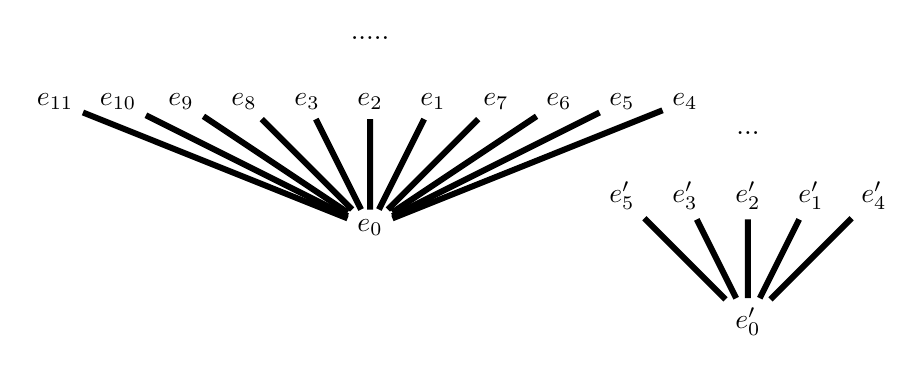
\begin{tikzpicture}[scale=0.4]
 				\node (I) at (-18,4) {$e_{11}$};
 				\node (J) at (-16,4) {$e_{10}$};
 				\node (K) at (-14,4) {$e_9$};
 				\node (L) at (-12,4) {$e_8$};
 				\node (A) at (-8,0) {$e_0$};
 				\node (B) at (-10,4) {$e_3$};
 				\node (C) at (-8,4) {$e_2$};
 					\node (C1) at (-8,6) {.....};
 				\node (D) at (-6,4) {$e_1$};
 				\node (E) at (-4,4) {$e_7$};
 				\node (F) at (-2,4) {$e_6$};
 				\node (G) at (0,4) {$e_5$};
 				\node (H) at (2,4) {$e_4$};
 				\draw[line width=.03in] (A) -- (B);
 				\draw[line width=.03in] (A) -- (C);
 				\draw[line width=.03in] (A) -- (D);
 				\draw[line width=.03in] (A) -- (E);
 				\draw[line width=.03in] (A) -- (F);
 				\draw[line width=.03in] (A) -- (G);
 				\draw[line width=.03in] (A) -- (H);
 				\draw[line width=.03in] (A) -- (I);
 				\draw[line width=.03in] (A) -- (J);
 				\draw[line width=.03in] (A) -- (K);
 				\draw[line width=.03in] (A) -- (L);
 
 				\node (A') at (4,-3) {$e_0'$};	
 					\node (B') at (0,1) {$e_5'$};
 					\node (C') at (2,1) {$e_3'$};
 					\node (D') at (4,1) {$e_2'$};
 						\node (D1') at (4,3) {...};
 					\node (E') at (6,1) {$e_1'$};
 					\node (F') at (8,1) {$e_4'$};
 				\draw[line width=.03in] (A') -- (B');
 				\draw[line width=.03in] (A') -- (C');
 				\draw[line width=.03in] (A') -- (D');
 				\draw[line width=.03in] (A') -- (E');
 				\draw[line width=.03in] (A') -- (F');	
 		\end{tikzpicture} \times 
 	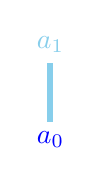
\begin{tikzpicture}[scale=0.4]
 				\node (A) at (0,0) {\textcolor{blue}{$a_0$}};
 				\node (B) at (0,3) {\textcolor{SkyBlue}{$a_1$}};
 				
 				\draw[SkyBlue, line width=.03in] (A) -- (B);
 				
 		\end{tikzpicture}} && 
 		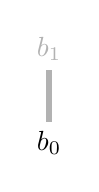
\begin{tikzpicture}[scale=0.4]
 			\node (A) at (0,0) {$b_0$};
 			\node (B) at (0,3) {\textcolor{gray!60}{$b_1$}};
 			
 			\draw[gray!60, line width=.03in] (A) -- (B);
 			
 		\end{tikzpicture} \\
 		\\
 		{\begin{tikzpicture}[thick,scale=0.45, every node/.style={scale=0.9}]
	 				\node (a)  at (-0.5,-0.5) {\textcolor{YellowOrange}{\bullet}};
	 				\node (A)  at (0,0) {\beta};
	 				\node (a')  at (0.5,-0.5) {\textcolor{blue}{\bullet}};	
	 					\node (b)  at (-0.5,2.5) {\textcolor{YellowOrange}{\bullet}};
	 					\node (B)  at (0,3) {\epsilon};
	 					\node (b')  at (0.5,2.5) {\textcolor{SkyBlue}{\bullet}};
	 				\node (c)  at (2.5,-0.5) {\textcolor{YellowOrange}{\bullet}};
	 				\node (C)  at (3,0) {\gamma};
	 				\node (c')  at (3.5,-0.5) {\textcolor{SkyBlue}{\bullet}};
	 				\node (d)  at (5.7,-0.5) {\textcolor{Bittersweet}{\bullet}};
	 				\node (D)  at (6,0) {\delta};
	 				\node (d')  at (6.5,-0.5) {\textcolor{SkyBlue}{\bullet}};
	 					\node (e)  at (5.5,2.5) {\textcolor{YellowOrange}{\bullet}};	
	 					\node (E)  at (6,3) {\zeta};
	 					\node (e')  at (6.5,2.5) {\textcolor{SkyBlue}{\bullet}};
 				\node (f)  at (2.5,-3.5) {\textcolor{Bittersweet}{\bullet}};
 				\node (F)  at (3,-3) {\alpha};
 				\node (f')  at (3.5,-3.5) {\textcolor{blue}{\bullet}};
 				
 				\draw [dotted] [line width=.03in] (A) -- (B);
 				\draw [dotted] [line width=.03in] (D) -- (E);
 				\draw [ line width=.03in] (F) -- (A);
 				\draw [ line width=.03in] (F) -- (C);
 				\draw [ line width=.03in] (F) -- (D);
 				
 		\end{tikzpicture}}
 		\arrow["g"', from=3-1, to=1-3]
 		\arrow["{\hat{g}\times id_A}"', from=3-1, to=1-1]
 		\arrow["eval"', from=1-1, to=1-3]
 	\end{tikzcd}
 	\caption{UMP diagram for $A=B=C=\textbf{1}_\bot$.  }
 \end{figure}
 \newline
(From now on the candidate for the exponential object in $\mathbb{FF}_3$ will be denoted by $"B^A"$ or simply by $B^A$). 
\newpage
The map \emph{eval} can be fully described as we saw in the case of Bushes. However we will concentrate our attention on a specific part of its domain in $"(\textbf{1}_\bot)^{\textbf{1}_\bot}" \times \textbf{1}_\bot$ namely the first levels of $T_0 \times \textbf{1}_\bot$ and display only this part in detail leaving the rest purposefully incomplete.
\begin{figure}[h]
	\begin{tikzcd}
		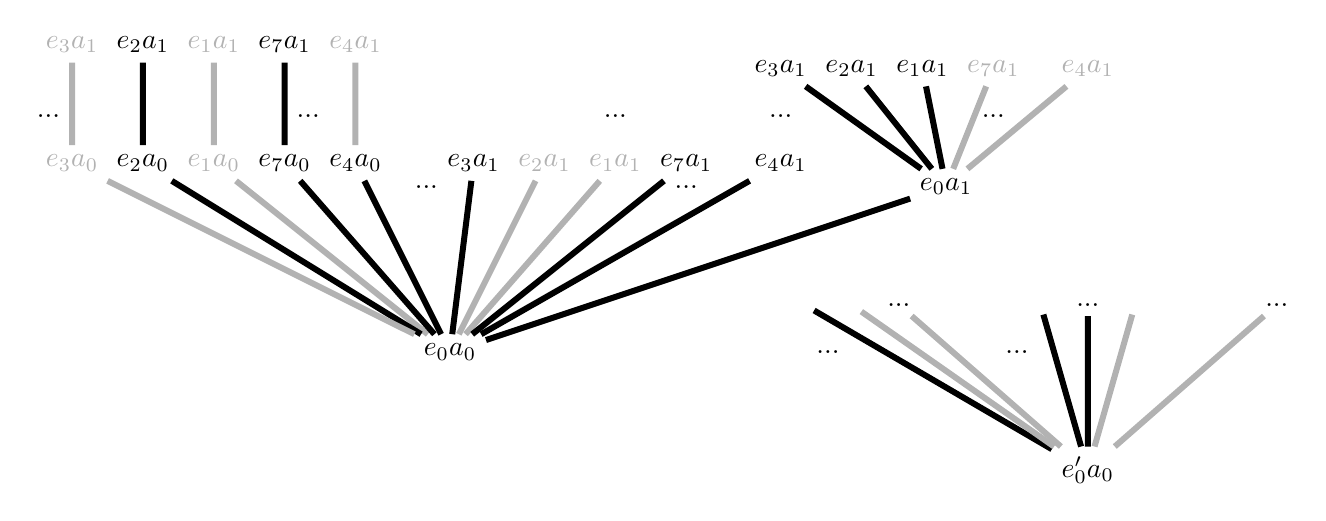
\begin{tikzpicture}[scale=0.3]
				\node (H') at (-35,5) {...};
			\node (H) at (-34,3) {\textcolor{gray!60}{$e_3 a_0$}};
				\node (H1) at (-34,8) {\textcolor{gray!60}{$e_3 a_1$}};
			\node (G) at (-31,3) {$e_2 a_0$};
				\node (G1) at (-31,8) {$e_2 a_1$};
			\node (F) at (-28,3) {\textcolor{gray!60}{$e_1 a_0$}};
				\node (F1) at (-28,8) {\textcolor{gray!60}{$e_1 a_1$}};
			\node (A3) at (-25,3) {$e_7 a_0$};	
				\node (A3') at (-25,8) {$e_7 a_1$};
				\node (A3'') at (-24,5) {...};
			\node (A4) at (-22,3) {$e_4 a_0$};	
				\node (A4') at (-22,8) {\textcolor{gray!60}{$e_4 a_1$}};	
			\node (A) at (-18,-5) {$e_0 a_0$};
				\node (B') at (-19,2) {...};
			\node (B) at (-17,3) {$e_3 a_1$};
			\node (C) at (-14,3) {\textcolor{gray!60}{$e_2 a_1$}};
			\node (D) at (-11,3) {\textcolor{gray!60}{$e_1 a_1$}};
				\node (D') at (-11,5) {...};
			\node (A1) at (-4,3) {$e_4 a_1$};
				\node (A1') at (-8,2) {...};
			\node (A2) at (-8,3) {$e_7 a_1$};
			\node (E) at (3,2) {$e_0 a_1$};
				\node (E1) at (9,7) {\textcolor{gray!60}{$e_4 a_1$}};
					\node (E1') at (5,5) {...};
				\node (E2) at (5,7) {\textcolor{gray!60}{$e_7 a_1$}};
				\node (E3) at (2,7) {$e_1 a_1$};
				\node (E4) at (-1,7) {$e_2 a_1$};	
				\node (E5) at (-4,7) {$e_3 a_1$};
					\node (E5') at (-4,5) {...};		
			\draw[line width=.03in] (A) -- (B);
			\draw[gray!60, line width=.03in] (A) -- (C);
			\draw[gray!60, line width=.03in] (A) -- (D);
			\draw[line width=.03in] (A) -- (A1);
			\draw[line width=.03in] (A) -- (A2);
			\draw[line width=.03in] (A) -- (E);
				\draw[gray!60, line width=.03in] (E) -- (E1);
				\draw[gray!60, line width=.03in] (E) -- (E2);
				\draw[line width=.03in] (E) -- (E3);
				\draw[line width=.03in] (E) -- (E4);
				\draw[line width=.03in] (E) -- (E5);
			\draw[gray!60, line width=.03in] (A) -- (F);
				\draw[gray!60, line width=.03in] (F) -- (F1);
			\draw[line width=.03in] (A) -- (A3);
				\draw[line width=.03in] (A3) -- (A3');
			\draw[line width=.03in] (A) -- (A4);
				\draw[gray!60, line width=.03in] (A4) -- (A4');	
			\draw[line width=.03in] (A) -- (G);
				\draw[line width=.03in] (G) -- (G1);
			\draw[gray!60, line width=.03in] (A) -- (H);
				\draw[gray!60, line width=.03in] (H) -- (H1);
		
				\node (M') at (-2,-5) {...};
			\node (H') at (-3,-3) {};
			\node (G') at (-1,-3) {};
			\node (F') at (1,-3) {...};
			\node (A') at (9,-10) {$e_0'a_0$};
				\node (N') at (6,-5) {...};
			\node (B') at (7,-3) {};
			\node (C') at (9,-3) {...};
			\node (D') at (11,-3) {};
			\node (E') at (17,-3) {...};
			\draw[line width=.03in] (A') -- (H');
			\draw[gray!60, line width=.03in] (A') -- (G');
			\draw[gray!60, line width=.03in] (A') -- (F');
			\draw[line width=.03in] (A') -- (B');
			\draw[line width=.03in] (A') -- (C');
			\draw[gray!60, line width=.03in] (A') -- (D');
			\draw[gray!60, line width=.03in] (A') -- (E');
			
			
		\end{tikzpicture} \\
		\\
		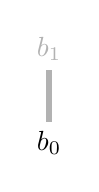
\begin{tikzpicture}[scale=0.3]
			\node (A) at (0,0) {$b_0$};
			\node (B) at (0,4) {\textcolor{gray!60}{$b_1$}};
			
			\draw[gray!60, line width=.03in] (A) -- (B);
		\end{tikzpicture}
		\arrow["eval"', from=1-1, to=3-1]
	\end{tikzcd}
	\caption{The map $eval : B^A \times A \rightarrow B : (\textbf{1}_\bot)^{\textbf{1}_\bot}\times \textbf{1}_\bot \rightarrow \textbf{1}_\bot$.\newline The pre-image of $b_1$ is colored in gray and that of $b_0$ in black. \newline
	In this case the nodes of the product are labeled with $e_ia_j$ to specify the left and right projections to $e_i$ and $a_j$ respectively.}
\end{figure}

\newpage
Remember that, as in the previous case for \emph{bushes}, we would like for the exponential object to encode the maps $\{ g_j \}_{j=0}^{17}$. The first two levels of $(\textbf{1}_\bot)^{\textbf{1}_\bot}$ can thus be labeled in a similar fashion as before. 

\begin{figure}[h]
	\centering
	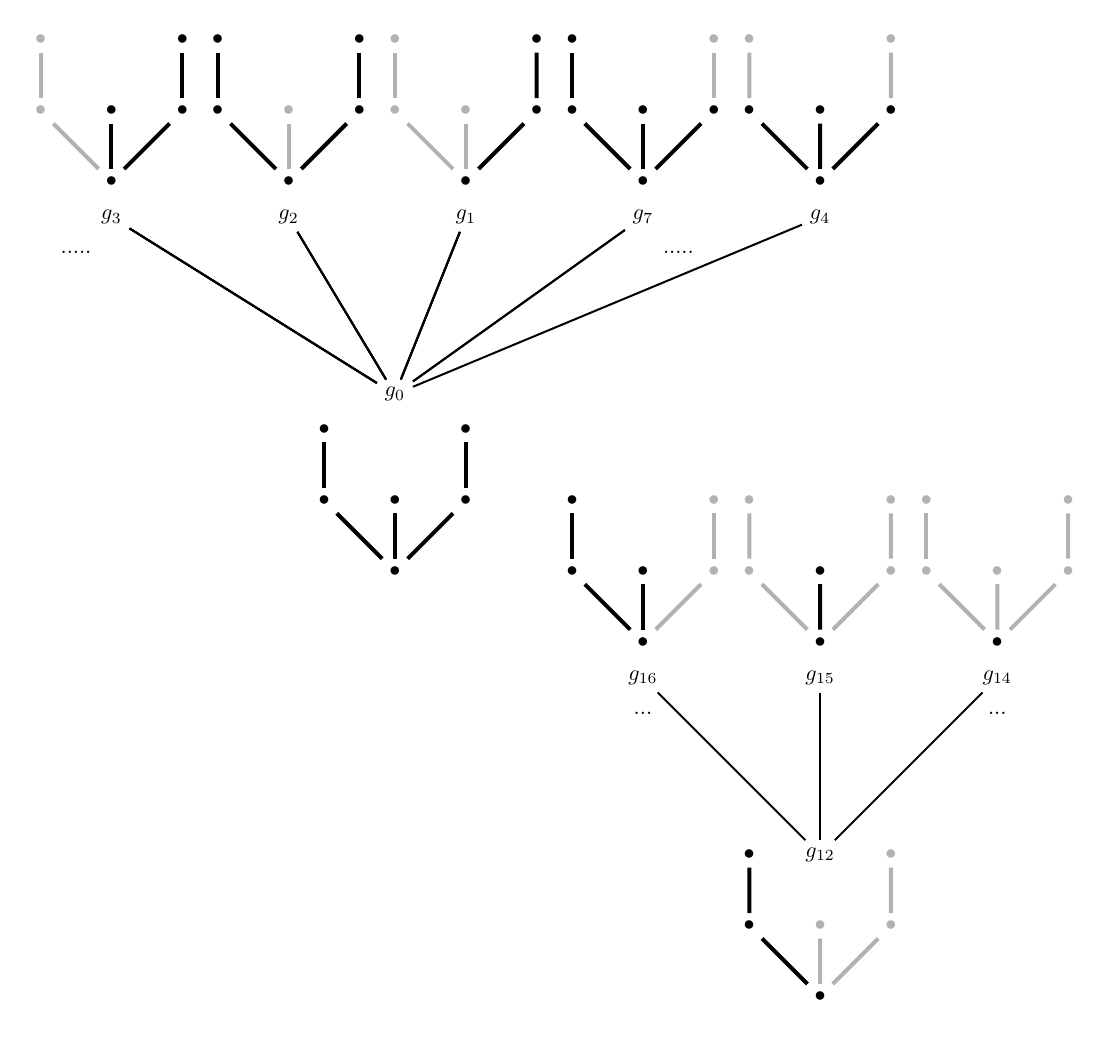
\begin{tikzpicture}[scale=0.45, every node/.style={scale=0.8}]
		\node (A) at (3,0) {$g_0$};
			\node (A0) at (3,-5) {\textcolor{black}{$\bullet$}};
			\node (B0) at (1,-3) {\textcolor{black}{$\bullet$}};
				\node (B0') at (1,-1) {\textcolor{black}{$\bullet$}};
			\node (C0) at (3,-3) {\textcolor{black}{$\bullet$}};
			\node (D0) at (5,-3) {\textcolor{black}{$\bullet$}};
				\node (D0') at (5,-1) {\textcolor{black}{$\bullet$}};
			\draw[line width=.02in] (A0) -- (B0);
				\draw[line width=.02in] (B0) -- (B0');
			\draw[line width=.02in] (A0) -- (C0);
			\draw[line width=.02in] (A0) -- (D0);
				\draw[line width=.02in] (D0) -- (D0');
		\node (B) at (-5,5) {$g_3$};
			\node (B') at (-6,4) {.....};
			\node (A3) at (-5,6) {\textcolor{black}{$\bullet$}};
				\node (B3) at (-7,8) {\textcolor{gray!60}{$\bullet$}};
					\node (B3') at (-7,10) {\textcolor{gray!60}{$\bullet$}};
				\node (C3) at (-5,8) {\textcolor{black}{$\bullet$}};
				\node (D3) at (-3,8) {\textcolor{black}{$\bullet$}};
						\node (D3') at (-3,10) {\textcolor{black}{$\bullet$}};
			\draw[gray!60, line width=.02in] (A3) -- (B3);
				\draw[gray!60, line width=.02in] (B3) -- (B3');
			\draw[line width=.02in] (A3) -- (C3);
			\draw[line width=.02in] (A3) -- (D3);
				\draw[line width=.02in] (D3) -- (D3');
		\node (C) at (0,5) {$g_2$};
			\node (A2) at (0,6) {\textcolor{black}{$\bullet$}};
				\node (B2) at (-2,8) {\textcolor{black}{$\bullet$}};
					\node (B2') at (-2,10) {\textcolor{black}{$\bullet$}};
				\node (C2) at (0,8) {\textcolor{gray!60}{$\bullet$}};
				\node (D2) at (2,8) {\textcolor{black}{$\bullet$}};
					\node (D2') at (2,10) {\textcolor{black}{$\bullet$}};
				\draw[line width=.02in] (A2) -- (B2);
					\draw[line width=.02in] (B2) -- (B2');
				\draw[gray!60, line width=.02in] (A2) -- (C2);
				\draw[line width=.02in] (A2) -- (D2);
					\draw[line width=.02in] (D2) -- (D2');
		\node (D) at (5,5) {$g_1$};
			\node (A1) at (5,6) {\textcolor{black}{$\bullet$}};
				\node (B1) at (3,8) {\textcolor{gray!60}{$\bullet$}};
					\node (B1') at (3,10) {\textcolor{gray!60}{$\bullet$}};
				\node (C1) at (5,8) {\textcolor{gray!60}{$\bullet$}};
				\node (D1) at (7,8) {\textcolor{black}{$\bullet$}};
					\node (D1') at (7,10) {\textcolor{black}{$\bullet$}};
				\draw[gray!60, line width=.02in] (A1) -- (B1);
					\draw[gray!60, line width=.02in] (B1) -- (B1');
				\draw[gray!60, line width=.02in] (A1) -- (C1);
				\draw[line width=.02in] (A1) -- (D1);
					\draw[line width=.02in] (D1) -- (D1');
				\draw[line width=.01in] (A) -- (B);
				\draw[line width=.01in] (A) -- (C);
				\draw[line width=.01in] (A) -- (D);
		\node (E) at (10,5) {$g_7$};
		\node (e) at (11,4) {.....};
			\node (A7) at (10,6) {\textcolor{black}{$\bullet$}};
				\node (B7) at (8,8) {\textcolor{black}{$\bullet$}};
					\node (B7') at (8,10) {\textcolor{black}{$\bullet$}};
				\node (C7) at (10,8) {\textcolor{black}{$\bullet$}};
				\node (D7) at (12,8) {\textcolor{black}{$\bullet$}};
					\node (D7') at (12,10) {\textcolor{gray!60}{$\bullet$}};
				\draw[line width=.02in] (A7) -- (B7);
					\draw[line width=.02in] (B7) -- (B7');
				\draw[line width=.02in] (A7) -- (C7);
				\draw[line width=.02in] (A7) -- (D7);
					\draw[gray!60, line width=.02in] (D7) -- (D7');
				\draw[line width=.01in] (A) -- (B);
				\draw[line width=.01in] (A) -- (C);
				\draw[line width=.01in] (A) -- (D);
				\draw[line width=.01in] (A) -- (E);
		\node (F) at (15,5) {$g_4$};
			\node (A4) at (15,6) {\textcolor{black}{$\bullet$}};
				\node (B4) at (13,8) {\textcolor{black}{$\bullet$}};
					\node (B4') at (13,10) {\textcolor{gray!60}{$\bullet$}};
				\node (C4) at (15,8) {\textcolor{black}{$\bullet$}};
				\node (D4) at (17,8) {\textcolor{black}{$\bullet$}};
					\node (D4') at (17,10) {\textcolor{gray!60}{$\bullet$}};
				\draw[line width=.02in] (A4) -- (B4);
					\draw[gray!60, line width=.02in] (B4) -- (B4');
				\draw[line width=.02in] (A4) -- (C4);
				\draw[line width=.02in] (A4) -- (D4);
					\draw[gray!60, line width=.02in] (D4) -- (D4');
		\draw[line width=.01in] (A) -- (B);
		\draw[line width=.01in] (A) -- (C);
		\draw[line width=.01in] (A) -- (D);
		\draw[line width=.01in] (A) -- (E);	
		\draw[line width=.01in] (A) -- (F);			
			
		\node (A') at (15,-13) {$g_{12}$};
			\node (A0') at (15,-17) {\textcolor{black}{$\bullet$}};
				\node (B0') at (13,-15) {\textcolor{black}{$\bullet$}};
					\node (B0'') at (13,-13) {\textcolor{black}{$\bullet$}};
				\node (C0') at (15,-15) {\textcolor{gray!60}{$\bullet$}};
				\node (D0') at (17,-15) {\textcolor{gray!60}{$\bullet$}};	
					\node (D0'') at (17,-13) {\textcolor{gray!60}{$\bullet$}};
			\draw[line width=.02in] (A0') -- (B0');
			\draw[line width=.02in] (B0') -- (B0'');
			\draw[gray!60, line width=.02in] (A0') -- (C0');
			\draw[gray!60, line width=.02in] (A0') -- (D0');
			\draw[gray!60, line width=.02in] (D0') -- (D0'');
		\node (B'') at (10,-9) {...};
		\node (B') at (10,-8) {$g_{16}$};
			\node (A1') at (10,-7) {\textcolor{black}{$\bullet$}};
				\node (B1') at (8,-5) {\textcolor{black}{$\bullet$}};
					\node (B1'') at (8,-3) {\textcolor{black}{$\bullet$}};
				\node (C1') at (10,-5) {\textcolor{black}{$\bullet$}};				
				\node (D1') at (12,-5) {\textcolor{gray!60}{$\bullet$}};
					\node (D1'') at (12,-3) {\textcolor{gray!60}{$\bullet$}};
			\draw[ line width=.02in] (A1') -- (B1');
				\draw[ line width=.02in] (B1') -- (B1'');
			\draw[ line width=.02in] (A1') -- (C1');
			\draw[gray!60, line width=.02in] (A1') -- (D1');
				\draw[gray!60, line width=.02in] (D1') -- (D1'');		
		\node (C') at (15,-8) {$g_{15}$};
			\node (A2') at (15,-7) {\textcolor{black}{$\bullet$}};
				\node (B2') at (13,-5) {\textcolor{gray!60}{$\bullet$}};
					\node (B2'') at (13,-3) {\textcolor{gray!60}{$\bullet$}};
				\node (C2') at (15,-5) {\textcolor{black}{$\bullet$}};
				\node (D2') at (17,-5) {\textcolor{gray!60}{$\bullet$}};
					\node (D2'') at (17,-3) {\textcolor{gray!60}{$\bullet$}};
				\draw[gray!60, line width=.02in] (A2') -- (B2');
					\draw[gray!60, line width=.02in] (B2') -- (B2'');
				\draw[line width=.02in] (A2') -- (C2');
				\draw[gray!60, line width=.02in] (A2') -- (D2');
					\draw[gray!60, line width=.02in] (D2') -- (D2'');		
		\node (D') at (20,-8) {$g_{14}$};
		\node (D'') at (20,-9) {...};
			\node (A3') at (20,-7) {\textcolor{black}{$\bullet$}};
				\node (B3') at (18,-5) {\textcolor{gray!60}{$\bullet$}};
						\node (B3'') at (18,-3) {\textcolor{gray!60}{$\bullet$}};
				\node (C3') at (20,-5) {\textcolor{gray!60}{$\bullet$}};
				\node (D3') at (22,-5) {\textcolor{gray!60}{$\bullet$}};
					\node (D3'') at (22,-3) {\textcolor{gray!60}{$\bullet$}};
				\draw[gray!60, line width=.02in] (A3') -- (B3');
					\draw[gray!60, line width=.02in] (B3') -- (B3'');
				\draw[gray!60, line width=.02in] (A3') -- (C3');
				\draw[gray!60, line width=.02in] (A3') -- (D3');
					\draw[gray!60, line width=.02in] (D3') -- (D3'');
		\draw[line width=.01in] (A') -- (B');
		\draw[line width=.01in] (A') -- (C');
		\draw[line width=.01in] (A') -- (D');
	\end{tikzpicture}
	\caption{The encoded maps  $\{ g_j \}_{j=0}^{17}$ in $(\textbf{1}_\bot) ^ {\textbf{1}_\bot}$. \newline
	Not all of them have been displayed.}
\end{figure}
\newpage
Now we take a new $C = (\textbf{1}_\bot)_\bot = \{c_0 < c_1 < c_2\}$ (which is just the old $C$ with a new \emph{child} $c_2$ of $c_1$) and consider maps from the new product $C \times A = (\textbf{1}_\bot)_\bot \times \textbf{1}_\bot$ to $B = \textbf{1}_\bot$.\newline
The following holds from Theorem~\ref{thm:prodffn}:
\begin{lem}
	For any $F,G \in \mathbb{FF}$ $F_\bot \times G$ is a super-forest of $F \times G$. 
\end{lem}
\begin{remark}
	We have seen that $\textbf{1}_\bot \times \textbf{1}_\bot \in \mathbb{FF}_3$ and so
	 $(\textbf{1}_\bot)_\bot \times_{\mathbb{FF}_3} \textbf{1}_\bot$ is a super-forest of $\textbf{1}_\bot \times \textbf{1}_\bot$.
\end{remark}
With this in mind, we examine the new UMP diagram in the $\mathbb{FF}_3$ environment
and introduce Greek letters to mark the nodes of $C \times A$ and left and right colored bullets
on the product to display the left and right projections. As before we use dotted lines to highlight the new branches of the super-forest.  
 \begin{figure}[h]
	\centering
	\begin{tikzcd}
		{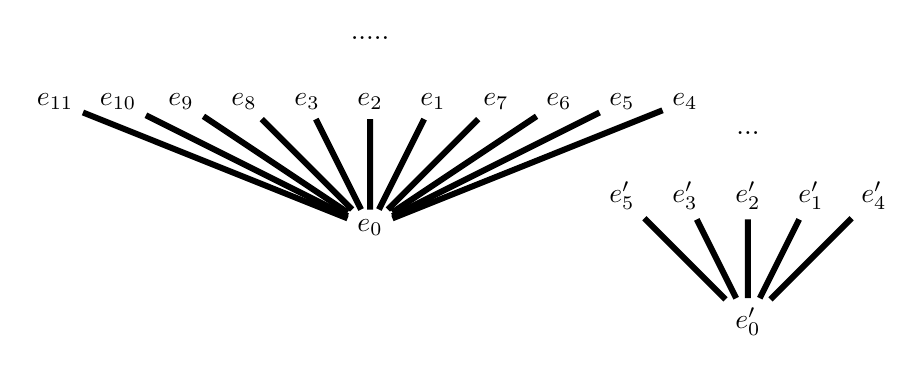
\begin{tikzpicture}[scale=0.4]
				\node (I) at (-18,4) {$e_{11}$};
				\node (J) at (-16,4) {$e_{10}$};
				\node (K) at (-14,4) {$e_9$};
				\node (L) at (-12,4) {$e_8$};
				\node (A) at (-8,0) {$e_0$};
				\node (B) at (-10,4) {$e_3$};
				\node (C) at (-8,4) {$e_2$};
				\node (C1) at (-8,6) {.....};
				\node (D) at (-6,4) {$e_1$};
				\node (E) at (-4,4) {$e_7$};
				\node (F) at (-2,4) {$e_6$};
				\node (G) at (0,4) {$e_5$};
				\node (H) at (2,4) {$e_4$};
				\draw[line width=.03in] (A) -- (B);
				\draw[line width=.03in] (A) -- (C);
				\draw[line width=.03in] (A) -- (D);
				\draw[line width=.03in] (A) -- (E);
				\draw[line width=.03in] (A) -- (F);
				\draw[line width=.03in] (A) -- (G);
				\draw[line width=.03in] (A) -- (H);
				\draw[line width=.03in] (A) -- (I);
				\draw[line width=.03in] (A) -- (J);
				\draw[line width=.03in] (A) -- (K);
				\draw[line width=.03in] (A) -- (L);
				
				\node (A') at (4,-3) {$e_0'$};	
				\node (B') at (0,1) {$e_5'$};
				\node (C') at (2,1) {$e_3'$};
				\node (D') at (4,1) {$e_2'$};
				\node (D1') at (4,3) {...};
				\node (E') at (6,1) {$e_1'$};
				\node (F') at (8,1) {$e_4'$};
				\draw[line width=.03in] (A') -- (B');
				\draw[line width=.03in] (A') -- (C');
				\draw[line width=.03in] (A') -- (D');
				\draw[line width=.03in] (A') -- (E');
				\draw[line width=.03in] (A') -- (F');	
			\end{tikzpicture} \times 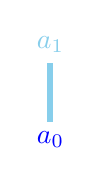
\begin{tikzpicture}[scale=0.4]
				\node (A) at (0,0) {\textcolor{blue}{$a_0$}};
				\node (B) at (0,3) {\textcolor{SkyBlue}{$a_1$}};
				
				\draw[SkyBlue, line width=.03in] (A) -- (B);
				
		\end{tikzpicture}} && 
		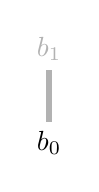
\begin{tikzpicture}[scale=0.4]
			\node (A) at (0,0) {$b_0$};
			\node (B) at (0,3) {\textcolor{gray!60}{$b_1$}};
			
			\draw[gray!60, line width=.03in] (A) -- (B);
			
		\end{tikzpicture} \\
		\\
			{\begin{tikzpicture}[thick,scale=0.45, every node/.style={scale=0.9}]
			\node (f')  at (2.5,-3.5) {\textcolor{Bittersweet}{\bullet}};
			\node (F)  at (3,-3) {\alpha};	
			\node (f)  at (3.5,-3.5) {\textcolor{blue}{\bullet}};
			\node (a')  at (-0.7,-0.5) {\textcolor{YellowOrange}{\bullet}};
			\node (A)  at (0,0) {\beta\;};
			\node (a)  at (0.3,-0.5) {\textcolor{blue}{\bullet}};
			\node (b')  at (-0.5,2.5) {\textcolor{YellowOrange}{\bullet}};
			\node (B)  at (0,3) {\eta};
			\node (f)  at (0.5,2.5) {\textcolor{SkyBlue}{\bullet}};
			\node (b1')  at (-3.5,2.5) {\textcolor{Lavender}{\bullet}};	
			\node (B1)  at (-3,3) {\zeta};
			\node (b1)  at (-2.5,2.5) {\textcolor{SkyBlue}{\bullet}};
			\node (b2')  at (-6.5,2.5) {\textcolor{Lavender}{\bullet}};
			\node (B2)  at (-6,3) {\epsilon};
			\node (b2)  at (-5.5,2.5) {\textcolor{blue}{\bullet}};
			\node (c')  at (2.5,-0.5) {\textcolor{YellowOrange}{\bullet}};		
			\node (C)  at (3,0) {\gamma};
			\node (c)  at (3.5,-0.5) {\textcolor{SkyBlue}{\bullet}};
			\node (c1')  at (2.5,2.5) {\textcolor{Lavender}{\bullet}};
			\node (C1)  at (3,3) {\theta};
			\node (c1)  at (3.5,2.5) {\textcolor{SkyBlue}{\bullet}};
			\node (d')  at (5.8,-0.5) {\textcolor{Bittersweet}{\bullet}};
			\node (D)  at (6,0) {\;\;\delta};
			\node (d)  at (6.8,-0.5) {\textcolor{SkyBlue}{\bullet}};
			\node (e')  at (5.5,2.5) {\textcolor{YellowOrange}{\bullet}};
			\node (E)  at (6,3) {\iota};
			\node (e)  at (6.5,2.5) {\textcolor{SkyBlue}{\bullet}};

			\draw [ line width=.03in] (F) -- (A);
			\draw [line width=.03in] (A) -- (B);
			\draw [dotted, line width=.03in] (A) -- (B1);
			\draw [dotted, line width=.03in] (A) -- (B2);
			\draw [ line width=.03in] (F) -- (C);
			\draw [dotted, line width=.03in] (C) -- (C1);
			\draw [ line width=.03in] (F) -- (D);
			\draw [line width=.03in] (D) -- (E);

	\end{tikzpicture}}
		\arrow["g"', from=3-1, to=1-3]
		\arrow["{\hat{g}\times id_A}"', from=3-1, to=1-1]
		\arrow["eval"', from=1-1, to=1-3]
	\end{tikzcd}
	\caption{UMP diagram for $A=\{ \textcolor{blue}{a_0} < \textcolor{SkyBlue}{a_1}\}$, $B=\{ \textcolor{black}{b_0} < \textcolor{gray!60}{b_1}\}$ \newline
		and $C=\{\textcolor{Bittersweet}{c_0} < \textcolor{YellowOrange}{c_1} < \textcolor{Lavender}{c_2}\}$.  }
\end{figure}

\begin{remark} 
	$(\textbf{1}_\bot)_\bot \times \textbf{1}_\bot = ( (\textbf{1}_\bot \times \textbf{1}_\bot) + (\textbf{1}_\bot \times \textbf{1}) + ( (\textbf{1}_\bot)_\bot \times \textbf{1} ))_\bot = ( (\textbf{1}_\bot \times \textbf{1}_\bot) + \textbf{1}_\bot +  (\textbf{1}_\bot)_\bot)_\bot$. Recall also that $(\textbf{1}_\bot)_\bot \times_{\mathbb{FF}_3} \textbf{1}_\bot$ is the sub-forest nodes of height at most 3.
\end{remark}
\newpage
We focus our attention now on maps from $C=\{c_0 < c_1 < c_2\} \times_{\mathbb{FF}_3} A=\{a_0 < a_1\}$ to $B= \{b_0 < b_1\}$ i.e., $C \times_{\mathbb{FF}_3} A = (\textbf{1}_\bot)_\bot \times_{\mathbb{FF}_3} \textbf{1}_\bot$ to $B = \textbf{1}_\bot$  that send every node of $\{c_0 < c_1 \} \times_{\mathbb{FF}_3} \{a_0 < a_1\}$ i.e., $\textbf{1}_\bot \times \textbf{1}_\bot$ to the root $b_0$.
We call these \emph{h-maps}.
\begin{definition}[\emph{h-map}]
	An h-map is a map $h:  (\textbf{1}_\bot)_\bot \times \textbf{1}_\bot \rightarrow \textbf{1}_\bot$ such that the sub-forest $\textbf{1}_\bot \times \textbf{1}_\bot  \text{ is mapped to the root of } \textbf{1}_\bot$.
\end{definition}

How many of these maps are there?

\begin{lem}
	There are in total 8 h-maps in $\mathbb{FF}_3$. 
\end{lem}

This is due to the fact that, once all the nodes of $\textbf{1}_\bot \times \textbf{1}_\bot$ are sent to the root, the remaining 3 nodes (labeled from left to right as $\epsilon,\zeta,\theta$) have no constraints and are incomparable, and are thus free to go to any of the 2 nodes of $\textbf{1}_\bot$ so $2^3=8$.
\newline

For example, one of these h-maps $h_1$ is:

\begin{figure}[h]
	\centering
	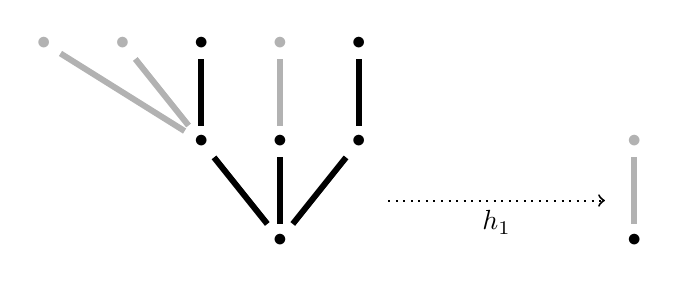
\begin{tikzpicture}[scale=0.25]
		
		\node (A) at (0,0) {$\textcolor{black}{\bullet}$};
		\node (B) at (-4,5) {$\textcolor{black}{\bullet}$};
		\node (B') at (-4,10) {$\textcolor{black}{\bullet}$};
		\node (B'') at (-8,10) {$\textcolor{gray!60}{\bullet}$};
		\node (B''') at (-12,10) {$\textcolor{gray!60}{\bullet}$};
		\node (C) at (0,5) {$\textcolor{black}{\bullet}$};
		\node (C') at (0,10) {$\textcolor{gray!60}{\bullet}$};
		\node (D) at (4,5) {$\textcolor{black}{\bullet}$};
		\node (D') at (4,10) {$\textcolor{black}{\bullet}$};
		\node (d) at (5,2) {};
		
		\draw[black, line width=.03in] (A) -- (B);
		\draw[black, line width=.03in] (B) -- (B');
		\draw[gray!60, line width=.03in] (B) -- (B'');
		\draw[gray!60, line width=.03in] (B) -- (B''');
		\draw[black, line width=.03in] (A) -- (C);
		\draw[line width=.03in] (A) -- (D);
		\draw[line width=.03in] (D) -- (D');
		\draw[gray!60, line width=.03in] (C) -- (C');
		
		\node (e) at (17,2) {};
		\node (E) at (18,0) {$\textcolor{black}{\bullet}$};
		\node (F) at (18,5) {$\textcolor{gray!60}{\bullet}$};
		\draw[gray!60, line width=.03in] (E) -- (F);
		
		\draw[->, dotted, line width=.01in] (d) -- node[anchor=north] {$h_1$} (e);
	\end{tikzpicture}
	
\end{figure}

How might these h-maps $\{h_i\}_{i=0}^7 : C \times A \rightarrow B$ be \emph{encoded} in the exponential $(\textbf{1}_\bot)^\textbf{1}_\bot$?
\newline\newline
Lets take a look at $\{\hat{h_i}\}_{i=0}^7 : C \rightarrow B^A$. 
\newline
Since $(\{c_0 < c_1\} = \textbf{1}_\bot) \times (\textbf{1}_\bot = \{a_0 < a_1\})$ is mapped by any $h_i$ to $b_0$ and this map (recall $g_0$) was already encoded, it follows from our previous work that
any $\hat{h_i}$ must send the nodes $c_0,c_1$ to the root $e_0$ of $B^A$. \newline 
What distinguishes these maps is the image of the node $c_2$  which can be any $e_i$, $i \in \{1,..,11\}$.
For example we can determine that  $\hat{h_0}: c_2 \mapsto e_0$ if we take $h_0$ as the h-map which sends every node of $C$ to the root $b_0$. 
\newline
A simple deduction is made from the fact that there are 8 h-maps that need to be encoded and at the same time there are 11 branches from the root $e_0$:
\begin{remark}
There are at least two distinct level-one  $i,j \in \{1,..,11\}$ $e_i,e_j$ nodes $i \neq j $ of $B^A$ that encode the same h-map $h_i$. 
We observe that the nodes $e_4$ and $e_7$ provide an example of this. 
\end{remark}
In other words: There are \emph{too many} branches for the h-maps. There are at least two distinct branches that encode the same h-map.
\newline
$C$ is again represented as $\{\textcolor{Bittersweet}{c_0} < \textcolor{YellowOrange}{c_1} < \textcolor{Lavender}{c_2}\}$ and the images of the nodes are displayed as bullets of the same color on $B^A$.
\begin{figure}[h]
	\centering
	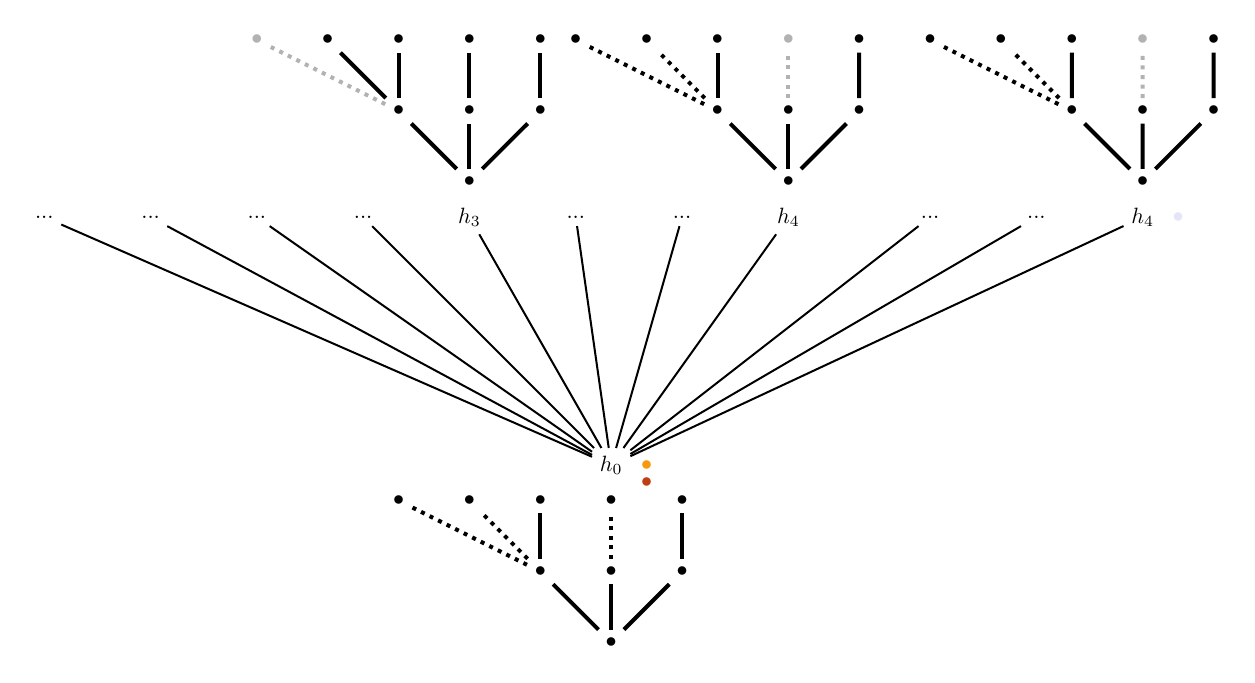
\begin{tikzpicture}[scale=0.45, every node/.style={scale=0.8}]
		\node (A) at (0,-2) {$h_0$};
			\node (A') at (1,-2.5) {\textcolor{Bittersweet}{$\bullet$}};
			\node (A'') at (1,-2) {\textcolor{YellowOrange}{$\bullet$}};
		\node (A0) at (0,-7) {\textcolor{black}{$\bullet$}};
			\node (B0) at (-2,-5) {\textcolor{black}{$\bullet$}};
				\node (B0') at (-2,-3) {\textcolor{black}{$\bullet$}};
				\node (B0'') at (-4,-3) {\textcolor{black}{$\bullet$}};
				\node (B0''') at (-6,-3) {\textcolor{black}{$\bullet$}};
			\node (C0) at (0,-5) {\textcolor{black}{$\bullet$}};
				\node (C0') at (0,-3) {\textcolor{black}{$\bullet$}};
			\node (D0) at (2,-5) {\textcolor{black}{$\bullet$}};
				\node (D0') at (2,-3) {\textcolor{black}{$\bullet$}};
			\draw[line width=.02in] (A0) -- (B0);
				\draw[line width=.02in] (B0) -- (B0');
				\draw[dotted, line width=.02in] (B0) -- (B0'');
				\draw[dotted, line width=.02in] (B0) -- (B0''');
			\draw[line width=.02in] (A0) -- (C0);
				\draw[dotted, line width=.02in] (C0) -- (C0');
			\draw[line width=.02in] (A0) -- (D0);
				\draw[line width=.02in] (D0) -- (D0');
		
		\node (L) at (-16,5) {...};
		
		\node (K) at (-13,5) {...};
		
		\node (J) at (-10,5) {...};
		
		\node (I) at (-7,5) {...};
		
		\node (B) at (-4,5) {$h_3$};
			\node (A3) at (-4,6) {\textcolor{black}{$\bullet$}};
				\node (B3) at (-6,8) {\textcolor{black}{$\bullet$}};
					\node (B3') at (-6,10) {\textcolor{black}{$\bullet$}};
					\node (B3'') at (-8,10) {\textcolor{black}{$\bullet$}};
					\node (B3''') at (-10,10) {\textcolor{gray!60}{$\bullet$}};
				\node (C3) at (-4,8) {\textcolor{black}{$\bullet$}};
					\node (C3') at (-4,10) {\textcolor{black}{$\bullet$}};
				\node (D3) at (-2,8) {\textcolor{black}{$\bullet$}};
					\node (D3') at (-2,10) {\textcolor{black}{$\bullet$}};
			\draw[line width=.02in] (A3) -- (B3);
					\draw[line width=.02in] (B3) -- (B3');
					\draw[line width=.02in] (B3) -- (B3'');
					\draw[dotted, gray!60, line width=.02in] (B3) -- (B3''');
				\draw[line width=.02in] (A3) -- (C3);
					\draw[line width=.02in] (C3) -- (C3');
				\draw[line width=.02in] (A3) -- (D3);
					\draw[line width=.02in] (D3) -- (D3');
		
		\node (C) at (-1,5) {...};
		
		\node (D) at (2,5) {...};
			
		\node (E) at (5,5) {$h_4$};
			\node (A7) at (5,6) {\textcolor{black}{$\bullet$}};
				\node (B7) at (3,8) {\textcolor{black}{$\bullet$}};
					\node (B7') at (3,10) {\textcolor{black}{$\bullet$}};
					\node (B7'') at (1,10) {\textcolor{black}{$\bullet$}};
					\node (B7''') at (-1,10) {\textcolor{black}{$\bullet$}};
				\node (C7) at (5,8) {\textcolor{black}{$\bullet$}};
						\node (C7') at (5,10) {\textcolor{gray!60}{$\bullet$}};
				\node (D7) at (7,8) {\textcolor{black}{$\bullet$}};
					\node (D7') at (7,10) {\textcolor{black}{$\bullet$}};
				\draw[line width=.02in] (A7) -- (B7);
					\draw[line width=.02in] (B7) -- (B7');
					\draw[dotted, line width=.02in] (B7) -- (B7'');
					\draw[dotted, line width=.02in] (B7) -- (B7''');
				\draw[line width=.02in] (A7) -- (C7);
					\draw[gray!60, dotted, line width=.02in] (C7) -- (C7');
				\draw[line width=.02in] (A7) -- (D7);
				\draw[line width=.02in] (D7) -- (D7');
				
		\node (H) at (9,5) {...};
		
		\node (G) at (12,5) {...};
		
		\node (F) at (15,5) {$h_4$};
			\node (F') at (16,5) {\textcolor{Lavender}{$\bullet$}};
			\node (A4) at (15,6) {\textcolor{black}{$\bullet$}};
				\node (B4) at (13,8) {\textcolor{black}{$\bullet$}};
					\node (B4') at (13,10) {\textcolor{black}{$\bullet$}};
					\node (B4'') at (11,10) {\textcolor{black}{$\bullet$}};
					\node (B4''') at (9,10) {\textcolor{black}{$\bullet$}};
				\node (C4) at (15,8) {\textcolor{black}{$\bullet$}};
					\node (C4') at (15,10) {\textcolor{gray!60}{$\bullet$}};
				\node (D4) at (17,8) {\textcolor{black}{$\bullet$}};
					\node (D4') at (17,10) {\textcolor{black}{$\bullet$}};
			\draw[line width=.02in] (A4) -- (B4);
				\draw[line width=.02in] (B4) -- (B4');
				\draw[dotted, line width=.02in] (B4) -- (B4'');
				\draw[dotted, line width=.02in] (B4) -- (B4''');
			\draw[line width=.02in] (A4) -- (C4);
				\draw[gray!60, dotted, line width=.02in] (C4) -- (C4');
			\draw[line width=.02in] (A4) -- (D4);
				\draw[line width=.02in] (D4) -- (D4');
			
			\draw[line width=.01in] (A) -- (B);
			\draw[line width=.01in] (A) -- (C);
			\draw[line width=.01in] (A) -- (D);
			\draw[line width=.01in] (A) -- (E);	
			\draw[line width=.01in] (A) -- (F);			
			\draw[line width=.01in] (A) -- (G);
			\draw[line width=.01in] (A) -- (H);
			\draw[line width=.01in] (A) -- (I);
			\draw[line width=.01in] (A) -- (J);
			\draw[line width=.01in] (A) -- (K);
			\draw[line width=.01in] (A) -- (L);
	\end{tikzpicture}
	\caption{Some of the encoded h-maps $\{\hat{h_i}\}_{i=0}^7 $ in $(\textbf{1}_\bot) ^ {\textbf{1}_\bot}$.}
\end{figure}

%\begin{figure}[h]
%	\centering
%	\begin{tikzcd}
%			\begin{tikzpicture}[scale=0.3, every node/.style={scale=0.8}]
%			\node (A) at (0,-3) {\textcolor{Bittersweet}{\bullet}};
%			\node (B) at (0,0) {\textcolor{YellowOrange}{\bullet}};
%			\node (C) at (0,3) {\textcolor{Lavender}{\bullet}};
%			\draw[line width=.01in] (A) -- (B);
%			\draw[line width=.01in] (B) -- (C);
%		\end{tikzpicture} && 	
%		\begin{tikzpicture}[scale=0.3, every node/.style={scale=0.8}]
%			\node (A) at (0,-2) {e_0};
%			\node (A') at (1,-2.5) {\textcolor{Bittersweet}{\bullet}};
%			\node (A'') at (1,-2) {\textcolor{YellowOrange}{\bullet}};
%			\node (L) at (-16,5) {e_{11}};
%			\node (K) at (-13,5) {e_{10}};
%			\node (J) at (-10,5) {e_9};
%			\node (I) at (-7,5) {e_8};
%			\node (B) at (-4,5) {e_3};
%			\node (C) at (-1,5) {e_2};
%			\node (c) at (-1,6.5) {.......};
%			\node (D) at (2,5) {e_1};
%			\node (E) at (5,5) {e_7};
%				\node (E') at (6,5) {\textcolor{Lavender}{\bullet}};
%			\node (H) at (9,5) {e_6};
%			\node (G) at (12,5) {e_5};
%			\node (F) at (15,5) {e_4};
%			\draw[line width=.01in] (A) -- (B);
%			\draw[line width=.01in] (A) -- (C);
%			\draw[line width=.01in] (A) -- (D);
%			\draw[line width=.01in] (A) -- (E);	
%			\draw[line width=.01in] (A) -- (F);			
%			\draw[line width=.01in] (A) -- (G);
%			\draw[line width=.01in] (A) -- (H);
%			\draw[line width=.01in] (A) -- (I);
%			\draw[line width=.01in] (A) -- (J);
%			\draw[line width=.01in] (A) -- (K);
%			\draw[line width=.01in] (A) -- (L);
%		\end{tikzpicture}
%		\arrow["{\hat{h}_j}",dotted, from=1-1, to=1-3]
%	\end{tikzcd}
%	\caption{}
%\end{figure}

What this entails is the following:
\begin{thm}\label{thm:ff3nottopos}
	$\mathbb{FF}_3$ is \emph{not} a topos.
\end{thm}
\begin{proof}
	Let us assume that $\mathbb{FF}_3$ is in fact a topos and admits exponential objects $F^G$ for all \emph{finite forests} $F,G$. \newline
	The example we just presented is evidence of the lack of uniqueness of adjoint h-maps $\hat{h} : (\textbf{1}_\bot)_\bot \rightarrow (\textbf{1}_\bot) ^ {\textbf{1}_\bot}$ that \emph{encode} $h :  (\textbf{1}_\bot)_\bot \times_{\mathbb{FF}_3} \textbf{1}_\bot \rightarrow \textbf{1}_\bot$.
	\newline
	Thus $(\textbf{1}_\bot) ^ {\textbf{1}_\bot}$ does not satisfy the UMP for the h-maps $h_i$.
	\newline
	Thus $\mathbb{FF}_3$ does not admit the exponential object $(\textbf{1}_\bot) ^ {\textbf{1}_\bot}$ and we conclude that it cannot be a topos.
\end{proof}
So there is a \emph{uniqueness} problem for exponentiation in $\mathbb{FF}_3$.
\newline
However $(\textbf{1}_\bot)_\bot \times_{\mathbb{FF}_3} \textbf{1}_\bot$ is a proper sub-forest of $(\textbf{1}_\bot)_\bot \times_{\mathbb{FF}} \textbf{1}_\bot$. 
\newline
How does the situation change if we consider $\mathbb{FF}_k$ with $k>3$ and $\mathbb{FF}$ in general?



\newpage
\subsection{\hl{Counter-example for $\mathbb{FF}_{k \geq 3}$}}

If we move on to $\mathbb{FF}_4$ or any $\mathbb{FF}_{k>3}$ we get the full product, not just a sub-forest of, $C \times A= (\textbf{1}_\bot)_\bot \times \textbf{1}_\bot$ given by  $( (\textbf{1}_\bot \times \textbf{1}_\bot) + \textbf{1}_\bot +  (\textbf{1}_\bot)_\bot)_\bot$.
\newline
As before we would like for the following UMP diagram to commute, use Greek letters to mark the nodes of $C \times A$ and colored bullets on the product for the projections.

\begin{figure}[h]
	\centering
	\begin{tikzcd}
		{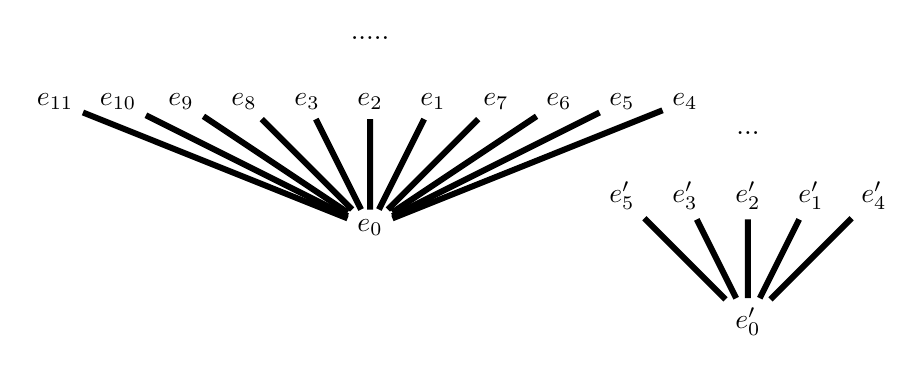
\begin{tikzpicture}[scale=0.4]
				\node (I) at (-18,4) {$e_{11}$};
				\node (J) at (-16,4) {$e_{10}$};
				\node (K) at (-14,4) {$e_9$};
				\node (L) at (-12,4) {$e_8$};
				\node (A) at (-8,0) {$e_0$};
				\node (B) at (-10,4) {$e_3$};
				\node (C) at (-8,4) {$e_2$};
				\node (C1) at (-8,6) {.....};
				\node (D) at (-6,4) {$e_1$};
				\node (E) at (-4,4) {$e_7$};
				\node (F) at (-2,4) {$e_6$};
				\node (G) at (0,4) {$e_5$};
				\node (H) at (2,4) {$e_4$};
				\draw[line width=.03in] (A) -- (B);
				\draw[line width=.03in] (A) -- (C);
				\draw[line width=.03in] (A) -- (D);
				\draw[line width=.03in] (A) -- (E);
				\draw[line width=.03in] (A) -- (F);
				\draw[line width=.03in] (A) -- (G);
				\draw[line width=.03in] (A) -- (H);
				\draw[line width=.03in] (A) -- (I);
				\draw[line width=.03in] (A) -- (J);
				\draw[line width=.03in] (A) -- (K);
				\draw[line width=.03in] (A) -- (L);
				
				\node (A') at (4,-3) {$e_0'$};	
				\node (B') at (0,1) {$e_5'$};
				\node (C') at (2,1) {$e_3'$};
				\node (D') at (4,1) {$e_2'$};
				\node (D1') at (4,3) {...};
				\node (E') at (6,1) {$e_1'$};
				\node (F') at (8,1) {$e_4'$};
				\draw[line width=.03in] (A') -- (B');
				\draw[line width=.03in] (A') -- (C');
				\draw[line width=.03in] (A') -- (D');
				\draw[line width=.03in] (A') -- (E');
				\draw[line width=.03in] (A') -- (F');	
			\end{tikzpicture} \times 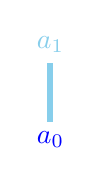
\begin{tikzpicture}[scale=0.4]
				\node (A) at (0,0) {\textcolor{blue}{$a_0$}};
				\node (B) at (0,3) {\textcolor{SkyBlue}{$a_1$}};
				
				\draw[SkyBlue, line width=.03in] (A) -- (B);
				
		\end{tikzpicture}} && 
		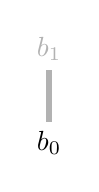
\begin{tikzpicture}[scale=0.4]
			\node (A) at (0,0) {$b_0$};
			\node (B) at (0,3) {\textcolor{gray!60}{$b_1$}};
			
			\draw[gray!60, line width=.03in] (A) -- (B);
			
		\end{tikzpicture} \\
		\\
		{\begin{tikzpicture}[thick,scale=0.5, every node/.style={scale=1.1}]
				\node (f')  at (2.5,-3.5) {\textcolor{Bittersweet}{\bullet}};
				\node (F)  at (3,-3) {\alpha};	
				\node (f)  at (3.5,-3.5) {\textcolor{blue}{\bullet}};
					\node (a')  at (-0.7,-0.5) {\textcolor{YellowOrange}{\bullet}};
					\node (A)  at (0,0) {\beta\;};
					\node (a)  at (0.3,-0.5) {\textcolor{blue}{\bullet}};
						\node (b')  at (-0.5,2.5) {\textcolor{YellowOrange}{\bullet}};
						\node (B)  at (0,3) {\eta};
						\node (f)  at (0.5,2.5) {\textcolor{SkyBlue}{\bullet}};
							\node (b'')  at (-0.5,5.5) {\textcolor{Lavender}{\bullet}};
							\node (B')  at (0,6) {\lambda};
							\node (b')  at (0.5,5.5) {\textcolor{SkyBlue}{\bullet}};
						\node (b1')  at (-3.5,2.5) {\textcolor{Lavender}{\bullet}};	
						\node (B1)  at (-3,3) {\zeta};
						\node (b1)  at (-2.5,2.5) {\textcolor{SkyBlue}{\bullet}};
						\node (b2')  at (-6.5,2.5) {\textcolor{Lavender}{\bullet}};
						\node (B2)  at (-6,3) {\epsilon};
						\node (b2)  at (-5.5,2.5) {\textcolor{blue}{\bullet}};
							\node (b2''')  at (-6.5,5.5) {\textcolor{Lavender}{\bullet}};
							\node (B2')  at (-6,6) {\kappa};
							\node (b2'')  at (-5.5,5.5) {\textcolor{SkyBlue}{\bullet}};
					\node (c')  at (2.5,-0.5) {\textcolor{YellowOrange}{\bullet}};		
					\node (C)  at (3,0) {\gamma};
					\node (c)  at (3.5,-0.5) {\textcolor{SkyBlue}{\bullet}};
						\node (c1')  at (2.5,2.5) {\textcolor{Lavender}{\bullet}};
						\node (C1)  at (3,3) {\theta};
						\node (c1)  at (3.5,2.5) {\textcolor{SkyBlue}{\bullet}};
					\node (d')  at (5.8,-0.5) {\textcolor{Bittersweet}{\bullet}};
					\node (D)  at (6,0) {\;\;\delta};
					\node (d)  at (6.8,-0.5) {\textcolor{SkyBlue}{\bullet}};
						\node (e')  at (5.5,2.5) {\textcolor{YellowOrange}{\bullet}};
						\node (E)  at (6,3) {\iota};
						\node (e)  at (6.5,2.5) {\textcolor{SkyBlue}{\bullet}};
							\node (e''')  at (5.5,5.5) {\textcolor{Lavender}{\bullet}};
							\node (E')  at (6,6) {\mu};
							\node (e'')  at (6.5,5.5) {\textcolor{SkyBlue}{\bullet}};
				\draw [ line width=.03in] (F) -- (A);
					\draw [line width=.03in] (A) -- (B);
						\draw [dotted, line width=.03in] (B) -- (B');
					\draw [dotted, line width=.03in] (A) -- (B1);
					\draw [dotted, line width=.03in] (A) -- (B2);
						\draw [dotted, line width=.03in] (B2) -- (B2');
				\draw [ line width=.03in] (F) -- (C);
					\draw [dotted, line width=.03in] (C) -- (C1);
				\draw [ line width=.03in] (F) -- (D);
					\draw [line width=.03in] (D) -- (E);
					\draw [dotted, line width=.03in] (E) -- (E');
	\end{tikzpicture}}
		\arrow["g"', from=3-1, to=1-3]
		\arrow["{\hat{g}\times id_A}"', from=3-1, to=1-1]
		\arrow["eval"', from=1-1, to=1-3]
	\end{tikzcd}
	\caption{UMP diagram for $A=\{ \textcolor{blue}{a_0} < \textcolor{SkyBlue}{a_1}\}$, $B=\{ \textcolor{black}{b_0} < \textcolor{gray!60}{b_1}\}$ and $C=\{\textcolor{Bittersweet}{c_0} < \textcolor{YellowOrange}{c_1} < \textcolor{Lavender}{c_2}\}$.   }
\end{figure}

As before we focus on \emph{h-maps} from $C \times A = (\textbf{1}_\bot)_\bot \times\textbf{1}_\bot$ to $B = \textbf{1}_\bot$.
	For example, one of these h-maps $h_1$ is:
\begin{figure}[h]
	\centering
	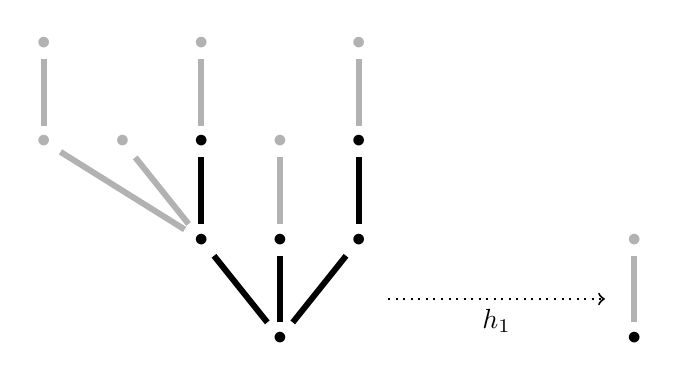
\begin{tikzpicture}[scale=0.25]
		
		\node (A) at (0,0) {$\textcolor{black}{\bullet}$};
		\node (B) at (-4,5) {$\textcolor{black}{\bullet}$};
		\node (B') at (-4,10) {$\textcolor{black}{\bullet}$};
		\node (B'''') at (-4,15) {$\textcolor{gray!60}{\bullet}$};
		\node (B'') at (-8,10) {$\textcolor{gray!60}{\bullet}$};
		\node (B''') at (-12,10) {$\textcolor{gray!60}{\bullet}$};
		\node (B''''') at (-12,15) {$\textcolor{gray!60}{\bullet}$};
		\node (C) at (0,5) {$\textcolor{black}{\bullet}$};
		\node (C') at (0,10) {$\textcolor{gray!60}{\bullet}$};
		\node (D) at (4,5) {$\textcolor{black}{\bullet}$};
		\node (D') at (4,10) {$\textcolor{black}{\bullet}$};
		\node (D'') at (4,15) {$\textcolor{gray!60}{\bullet}$};
		\node (d) at (5,2) {};
		
		\draw[black, line width=.03in] (A) -- (B);
		\draw[black, line width=.03in] (B) -- (B');
		\draw[gray!60, line width=.03in] (B') -- (B'''');
		\draw[gray!60, line width=.03in] (B) -- (B'');
		\draw[gray!60, line width=.03in] (B) -- (B''');
		\draw[gray!60, line width=.03in] (B''') -- (B''''');
		\draw[black, line width=.03in] (A) -- (C);
		\draw[line width=.03in] (A) -- (D);
		\draw[line width=.03in] (D) -- (D');
		\draw[gray!60, line width=.03in] (D') -- (D'');
		\draw[gray!60, line width=.03in] (C) -- (C');
		
		\node (e) at (17,2) {};
		\node (E) at (18,0) {$\textcolor{black}{\bullet}$};
		\node (F) at (18,5) {$\textcolor{gray!60}{\bullet}$};
		\draw[gray!60, line width=.03in] (E) -- (F);
		
		\draw[->, dotted, line width=.01in] (d) -- node[anchor=north] {$h_1$} (e);
	\end{tikzpicture}
	
\end{figure}

We ask again: How many of these maps are there?
\begin{lem}
There are in total 48 \emph{h-maps} in $\mathbb{FF}_{k > 3}$. 
\end{lem}

This can be computed by observing that compared to last time in $\mathbb{FF}_3$ we now have 3 new nodes to add to $C \times A$ so that $48=3 \cdot 2^4$.
\newline
The first one (reading the forest from left to right) $\kappa$ is the child of $\epsilon$, the second one $\lambda$ is the child of $\eta$ and the third one $\mu$ is the child of $\iota$.
If we observe the dotted branches we now have (still from left to right) one branch of the form $(\textbf{1}_\bot)_\bot$ and four of the form $(\textbf{1}_\bot)$. 
\newline
Recalling that $| Hom((\textbf{1}_\bot)_\bot, \textbf{1}_\bot) | =3$ and $| Hom(\textbf{1}_\bot, \textbf{1}_\bot) | =2$
a straightforward combinatorial argument tells us that the total number of \emph{h-maps} is $3 \cdot 2^4$.
\newline
 We ask again:
 How might these h-maps $\{h_i\}_{i=0}^{47} : C \times A \rightarrow B$ be \emph{encoded} in the exponential $(\textbf{1}_\bot)^{\textbf{1}_\bot}$?  \newline\newline
Lets take a look then at $\{\hat{h_i}\}_{i=0}^{47} : C \rightarrow B^A$. 
 \newline
The same argument we used last time tells us that any $\hat{h_i}$ must send the nodes $c_0,c_1$ to the root $e_0$ of $B^A$ and these maps should be distinguished by the image of the node $c_2$ which can be any $e_i$, $i \in \{1,..,11\}$.
 \newline
  Using the same example, we can determine that  $\hat{h_0}: c_2 \mapsto e_0$ if we take $h_0$ as the h-map which sends every node of $C$ to the root $b_0$.
  \newline
  In this case however there are 48 maps that need to be encoded with the same 11 branches from the root $e_0$.
   \newline
  This means that there are too \emph{few} branches to encode all the possible h-maps.
  
 \begin{lem}
 	There is at least one h-map that cannot be encoded in any level-one node $e_i$, $i \in \{0,..,11\}$ of $(\textbf{1}_\bot)^{\textbf{1}_\bot}$.
 \end{lem}
 The h-map $?h$ displayed in figure~\ref{fig:counterex} is an example of this.
  \newline
Let $\{\hat{h_i}\}_{i=1}^{11}$ be the maps from $C$ to $B^A$ such that $\hat{h_i}: \{c_0,c_1\}\mapsto e_0$ and $c_2 \mapsto e_i$. 
\newline
Take for example the h-map $h_7$ in display.
\newline
It should be in $1:1$ correspondence with $\hat{h_7}$.\newline 
Note that if we now focus our attention on $\{\beta < \eta < \lambda, \beta < \zeta,  \beta < \epsilon < \kappa\}$ i.e., the up-set $\uparrow \beta$ corresponding to $\{c_1 < c_2\} \times \{a_0 < a_1\}  $, the restriction of $\hat{h_7}$ already encodes a map which we called $g_7 :  \{c_1 < c_2\} \times \{a_0 < a_1\} \rightarrow \{b_0 < b_1\}$. \newline 
The yellow boxes in figure~\ref{fig:counterex} are meant to highlight this map. \newline	
If we construct a new h-map $?h$ which behaves exactly as $g_7$ on $\{c_1 < c_2\} \times \{a_0 < a_1\}$ but behaves differently on the two \emph{leaf} nodes $\theta, \mu$, then $?h \neq h_7$ and thus cannot be encoded by $\hat{h_7}$. \newline
Furthermore, $?h$ cannot be encoded by $\hat{h_i}$ with $i \neq 7$ since any of these $h_i$ when restricted to $\{c_1 < c_2\} \times \{a_0 < a_1\}$ behaves as $g_i$ with $g_i \neq g_7$.
\newline\newline
 We are thus in a bind and cannot find a corresponding $\hat{?h}$ for $?h$...
 \begin{figure}[h]
 	\centering
 	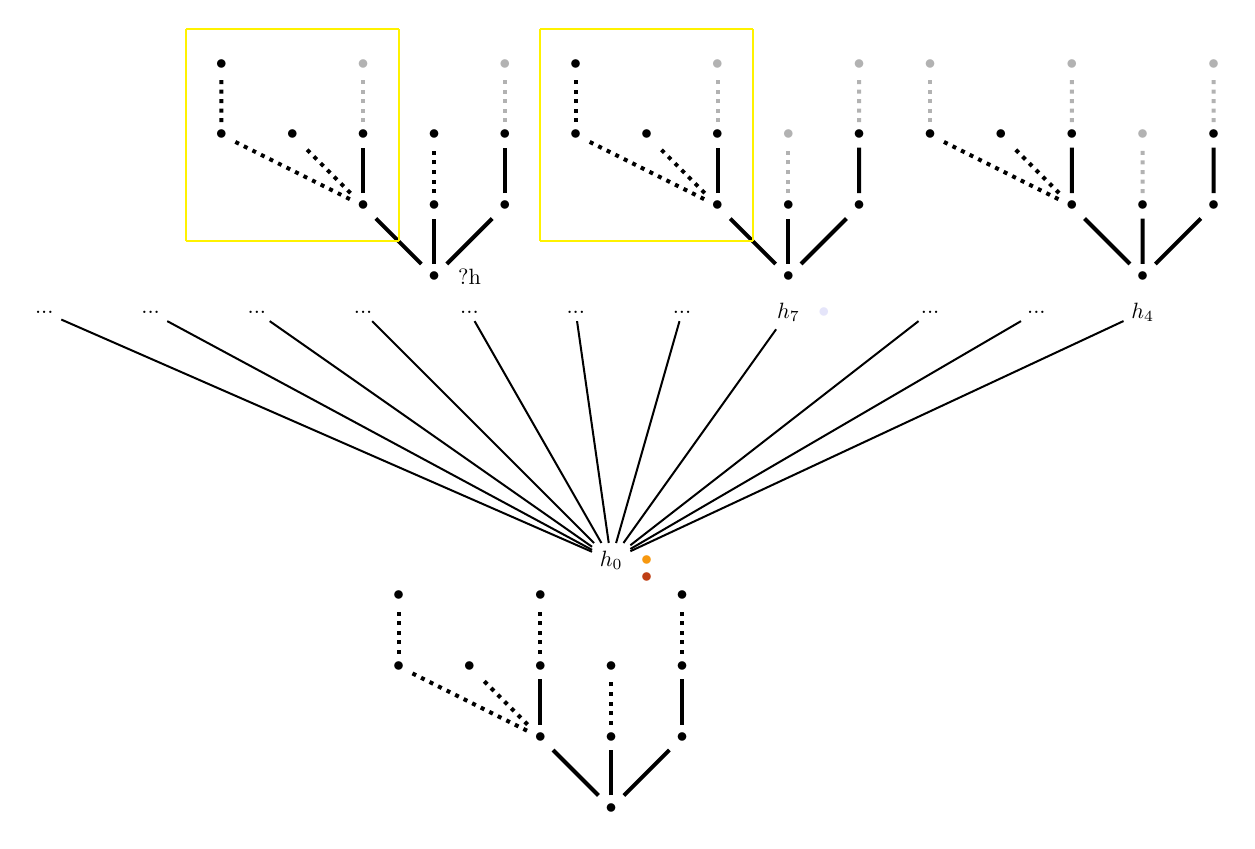
\begin{tikzpicture}[scale=0.45, every node/.style={scale=0.8}]
 		\node (A) at (0,-2) {$h_0$};
 		\node (A') at (1,-2.5) {\textcolor{Bittersweet}{$\bullet$}};
 		\node (A'') at (1,-2) {\textcolor{YellowOrange}{$\bullet$}};
	 	\node (A0) at (0,-9) {\textcolor{black}{$\bullet$}};
	 		\node (B0) at (-2,-7) {\textcolor{black}{$\bullet$}};
	 			\node (B0') at (-2,-5) {\textcolor{black}{$\bullet$}};
	 				\node (B0''''') at (-2,-3) {\textcolor{black}{$\bullet$}};
	 			\node (B0'') at (-4,-5) {\textcolor{black}{$\bullet$}};
	 			\node (B0''') at (-6,-5) {\textcolor{black}{$\bullet$}};
	 				\node (B0'''') at (-6,-3) {\textcolor{black}{$\bullet$}};
	 		\node (C0) at (0,-7) {\textcolor{black}{$\bullet$}};
	 			\node (C0') at (0,-5) {\textcolor{black}{$\bullet$}};
	 		\node (D0) at (2,-7) {\textcolor{black}{$\bullet$}};
	 			\node (D0') at (2,-5) {\textcolor{black}{$\bullet$}};
	 				\node (D0'') at (2,-3) {\textcolor{black}{$\bullet$}};
	 		\draw[line width=.02in] (A0) -- (B0);
		 		\draw[line width=.02in] (B0) -- (B0');
		 			\draw[dotted, line width=.02in] (B0') -- (B0''''');
		 		\draw[dotted, line width=.02in] (B0) -- (B0'');
		 		\draw[dotted, line width=.02in] (B0) -- (B0''');
		 			\draw[dotted, line width=.02in] (B0''') -- (B0'''');
		 	\draw[line width=.02in] (A0) -- (C0);
	 			\draw[dotted, line width=.02in] (C0) -- (C0');
	 		\draw[line width=.02in] (A0) -- (D0);
	 			\draw[line width=.02in] (D0) -- (D0');
					\draw[dotted, line width=.02in] (D0') -- (D0'');
		 		
 		\node (L) at (-16,5) {...};
 		
 		\node (K) at (-13,5) {...};
 		
 		\node (J) at (-10,5) {...};
 		
 		\node (I) at (-7,5) {...};
 		
 		\node (B) at (-4,5) {...};
 			\node (A3) at (-5,6) {\textcolor{black}{$\bullet$}};
	 		\node (A3') at (-4,6) {?h};
		 		\node (B3) at (-7,8) {\textcolor{black}{$\bullet$}};
		 			\node (B3') at (-7,10) {\textcolor{black}{$\bullet$}};
		 				\node (B3'''') at (-7,12) {\textcolor{gray!60}{$\bullet$}};
		 			\node (B3'') at (-9,10) {\textcolor{black}{$\bullet$}};
		 			\node (B3''') at (-11,10) {\textcolor{black}{$\bullet$}};
		 				\node (B3''''') at (-11,12) {\textcolor{black}{$\bullet$}};
		 		\node (C3) at (-5,8) {\textcolor{black}{$\bullet$}};
		 			\node (C3') at (-5,10) {\textcolor{black}{$\bullet$}};
		 		\node (D3) at (-3,8) {\textcolor{black}{$\bullet$}};
		 			\node (D3') at (-3,10) {\textcolor{black}{$\bullet$}};
		 				\node (D3'') at (-3,12) {\textcolor{gray!60}{$\bullet$}};
	 		\draw[line width=.02in] (A3) -- (B3);
	 			\draw[line width=.02in] (B3) -- (B3');
	 				\draw[dotted, gray!60, line width=.02in] (B3') -- (B3'''');
	 			\draw[dotted, line width=.02in] (B3) -- (B3'');
	 			\draw[dotted, line width=.02in] (B3) -- (B3''');
	 					\draw[dotted, line width=.02in] (B3''') -- (B3''''');
	 		\draw[line width=.02in] (A3) -- (C3);
	 			\draw[dotted, line width=.02in] (C3) -- (C3');
	 		\draw[line width=.02in] (A3) -- (D3);
	 			\draw[line width=.02in] (D3) -- (D3');
 					\draw[dotted, gray!60, line width=.02in] (D3') -- (D3'');
 			\draw[yellow, line width=.01in] (-6,7) -- (-6,13);
 			\draw[yellow, line width=.01in] (-6,13) -- (-12,13);
 			\draw[yellow, line width=.01in] (-12,13) -- (-12,7);
 			\draw[yellow, line width=.01in] (-12,7) -- (-6,7);
 			
 		\node (C) at (-1,5) {...};
 		
 		\node (D) at (2,5) {...};
 		
 		\node (E) at (5,5) {$h_7$};
 		 \node (E') at (6,5) {\textcolor{Lavender}{$\bullet$}};
 		\node (A7) at (5,6) {\textcolor{black}{$\bullet$}};
	 		\node (B7) at (3,8) {\textcolor{black}{$\bullet$}};
	 			\node (B7') at (3,10) {\textcolor{black}{$\bullet$}};
	 				\node (B7'''') at (3,12) {\textcolor{gray!60}{$\bullet$}};
	 			\node (B7'') at (1,10) {\textcolor{black}{$\bullet$}};
	 			\node (B7''') at (-1,10) {\textcolor{black}{$\bullet$}};
	 				\node (B7''''') at (-1,12) {\textcolor{black}{$\bullet$}};
	 		\node (C7) at (5,8) {\textcolor{black}{$\bullet$}};
	 			\node (C7') at (5,10) {\textcolor{gray!60}{$\bullet$}};
	 		\node (D7) at (7,8) {\textcolor{black}{$\bullet$}};
	 			\node (D7') at (7,10) {\textcolor{black}{$\bullet$}};
	 				\node (D7'') at (7,12) {\textcolor{gray!60}{$\bullet$}};
	 		\draw[line width=.02in] (A7) -- (B7);
	 			\draw[line width=.02in] (B7) -- (B7');
	 				\draw[dotted, gray!60, line width=.02in] (B7') -- (B7'''');
	 			\draw[dotted, line width=.02in] (B7) -- (B7'');
	 			\draw[dotted, line width=.02in] (B7) -- (B7''');
	 				\draw[dotted, line width=.02in] (B7''') -- (B7''''');
	 		\draw[line width=.02in] (A7) -- (C7);
	 			\draw[gray!60, dotted, line width=.02in] (C7) -- (C7');
	 		\draw[line width=.02in] (A7) -- (D7);
	 			\draw[line width=.02in] (D7) -- (D7');
	 				\draw[dotted, gray!60, line width=.02in] (D7') -- (D7'');
	 		\draw[yellow, line width=.01in] (4,7) -- (4,13);
	 		\draw[yellow, line width=.01in] (4,13) -- (-2,13);
	 		\draw[yellow, line width=.01in] (-2,13) -- (-2,7);
	 		\draw[yellow, line width=.01in] (-2,7) -- (4,7);
	 		
 		\node (H) at (9,5) {...};
 		
 		\node (G) at (12,5) {...};
 		
 		\node (F) at (15,5) {$h_4$};
	 		\node (A4) at (15,6) {\textcolor{black}{$\bullet$}};
		 		\node (B4) at (13,8) {\textcolor{black}{$\bullet$}};
		 			\node (B4') at (13,10) {\textcolor{black}{$\bullet$}};
		 					\node (B4'''') at (13,12) {\textcolor{gray!60}{$\bullet$}};
		 		\node (B4'') at (11,10) {\textcolor{black}{$\bullet$}};
		 		\node (B4''') at (9,10) {\textcolor{black}{$\bullet$}};
		 			\node (B4''''') at (9,12) {\textcolor{gray!60}{$\bullet$}};
		 		\node (C4) at (15,8) {\textcolor{black}{$\bullet$}};
		 			\node (C4') at (15,10) {\textcolor{gray!60}{$\bullet$}};
		 		\node (D4) at (17,8) {\textcolor{black}{$\bullet$}};
		 			\node (D4') at (17,10) {\textcolor{black}{$\bullet$}};
		 				\node (D4'') at (17,12) {\textcolor{gray!60}{$\bullet$}};
	 		\draw[line width=.02in] (A4) -- (B4);
	 			\draw[line width=.02in] (B4) -- (B4');
	 				\draw[gray!60, dotted, line width=.02in] (B4') -- (B4'''');
	 			\draw[dotted, line width=.02in] (B4) -- (B4'');
	 			\draw[dotted, line width=.02in] (B4) -- (B4''');
	 				\draw[gray!60, dotted, line width=.02in] (B4''') -- (B4''''');
	 		\draw[line width=.02in] (A4) -- (C4);
	 			\draw[gray!60, dotted, line width=.02in] (C4) -- (C4');
	 		\draw[line width=.02in] (A4) -- (D4);
	 			\draw[line width=.02in] (D4) -- (D4');
 					\draw[gray!60, dotted, line width=.02in] (D4') -- (D4'');
 		\draw[line width=.01in] (A) -- (B);
 		\draw[line width=.01in] (A) -- (C);
 		\draw[line width=.01in] (A) -- (D);
 		\draw[line width=.01in] (A) -- (E);	
 		\draw[line width=.01in] (A) -- (F);			
 		\draw[line width=.01in] (A) -- (G);
 		\draw[line width=.01in] (A) -- (H);
 		\draw[line width=.01in] (A) -- (I);
 		\draw[line width=.01in] (A) -- (J);
 		\draw[line width=.01in] (A) -- (K);
 		\draw[line width=.01in] (A) -- (L);
 		
 	\end{tikzpicture}
 	\caption{Some of the encoded h-maps $\{\hat{h_i}\}_{i=0}^{47} $ in $(\textbf{1}_\bot) ^ {\textbf{1}_\bot}$.}
 \label{fig:counterex}
 \end{figure}
 \newpage
 What this entails is the following:
 \begin{thm}\label{thm:ffknotatopos}
 	$\mathbb{FF}_{k > 3}$ for $k>3$ is \emph{not} a topos.
 \end{thm}
 \begin{proof}
 	Let us assume that $\mathbb{FF}_k$ is a topos for some $k > 3$ and admits exponential objects $F^G$ for all \emph{finite forests} $F,G$. 
\newline
 	The example we presented is evidence of the lack of existence of an adjoint h-map $\hat{h} : (\textbf{1}_\bot)_\bot \rightarrow (\textbf{1}_\bot) ^ {\textbf{1}_\bot}$ that \emph{encodes} $h :  (\textbf{1}_\bot)_\bot \times_{\mathbb{FF}_3} \textbf{1}_\bot \rightarrow \textbf{1}_\bot$. 
 	\newline
 	Thus $(\textbf{1}_\bot) ^ {\textbf{1}_\bot}$ does not satisfy the UMP for the h-maps $h_i$.
  \newline
 	Thus $\mathbb{FF}_k$ does not admit the exponential object $(\textbf{1}_\bot) ^ {\textbf{1}_\bot}$ and we conclude that it cannot be a topos.
 \end{proof}
 
 Summing up we have \emph{uniqueness} (Theorem~\ref{thm:ff3nottopos}) and \emph{existence} (Theorem~\ref{thm:ffknotatopos}) problems for exponentiation in $\mathbb{FF}_3$ and $\mathbb{FF}_{k> 3}$ respectively. The following results are now immediate:
 
 \begin{cor}
 	$\mathbb{FF}_{k\geq3}$ is not a topos.
 \end{cor}
 
 \begin{cor}
 	The only topoi in $\mathbb{FF}_*$ are $\mathbb{FF}_1 $ and $\mathbb{FF}_2$.
 \end{cor}



	\newpage
${}$ \newpage













